% !TEX TS-program = pdflatex
% !TEX encoding = UTF-8 Unicode

% This is a simple template for a LaTeX document using the "article" class.
% See "book", "report", "letter" for other types of document.

\documentclass[10pt]{article} % use larger type; default would be 10pt

\usepackage[utf8]{inputenc} % set input encoding (not needed with XeLaTeX)

%%% Examples of Article customizations
% These packages are optional, depending whether you want the features they provide.
% See the LaTeX Companion or other references for full information.

%%% PAGE DIMENSIONS
\usepackage{geometry} % to change the page dimensions
\geometry{letterpaper} % or letterpaper (US) or a5paper or....
\geometry{margin=1in} % for example, change the margins to 2 inches all round
% \geometry{landscape} % set up the page for landscape
%   read geometry.pdf for detailed page layout information

\usepackage{graphicx} % support the \includegraphics command and options
\usepackage{mathrsfs}
% \usepackage[parfill]{parskip} % Activate to begin paragraphs with an empty line rather than an indent

%%% PACKAGES
\usepackage{booktabs} % for much better looking tables
\usepackage{array} % for better arrays (eg matrices) in maths
\usepackage{paralist} % very flexible & customisable lists (eg. enumerate/itemize, etc.)
\usepackage{verbatim} % adds environment for commenting out blocks of text & for better verbatim
\usepackage{subfig} % make it possible to include more than one captioned figure/table in a single float
\usepackage[font=small,labelfont=bf]{caption} % Required for specifying captions to tables and figures
% These packages are all incorporated in the memoir class to one degree or another...

%%% HEADERS & FOOTERS
\usepackage{fancyhdr} % This should be set AFTER setting up the page geometry
\pagestyle{fancy} % options: empty , plain , fancy
\renewcommand{\headrulewidth}{0pt} % customise the layout...
\lhead{}\chead{}\rhead{}
\lfoot{}\cfoot{\thepage}\rfoot{}

%%% SECTION TITLE APPEARANCE
\usepackage{sectsty}
\allsectionsfont{\sffamily\mdseries\upshape} % (See the fntguide.pdf for font help)
% (This matches ConTeXt defaults)

%%% ToC (table of contents) APPEARANCE
\usepackage[nottoc,notlof,notlot]{tocbibind} % Put the bibliography in the ToC
\usepackage[titles,subfigure]{tocloft} % Alter the style of the Table of Contents
\renewcommand{\cftsecfont}{\rmfamily\mdseries\upshape}
\renewcommand{\cftsecpagefont}{\rmfamily\mdseries\upshape} % No bold!
\newcommand{\centerfig}[2]{\begin{center}\includegraphics[width=#1\textwidth]{#2}\end{center}}
\usepackage{amssymb}
\usepackage{mathtools}
\DeclarePairedDelimiter\ceil{\lceil}{\rceil}
\DeclarePairedDelimiter\floor{\lfloor}{\rfloor}
\let\oldemptyset\emptyset
\let\emptyset\varnothing
\usepackage[usenames, dvipsnames]{color}
\makeatletter
\def\@maketitle{%
  \newpage
  \null
  \vskip 1em%
  \begin{center}%
  \let \footnote \thanks
	\vskip -5em%
    {\LARGE \@title \par}%
    \vskip 1em
    {\large
      \lineskip .5em%
      \begin{tabular}[t]{c}%
        \@author
      \end{tabular}\par}%
    \vskip 1em%
    {\large \@date}%
  \end{center}%
  \par
  \vskip 1.5em}
\makeatother
%%% END Article customizations

%%% The "real" document content comes below...

\title{Physics 410: Project 3}
\author{Arnold Choa -- 32038144}
\date{12 November, 2018} % Activate to display a given date or no date (if empty),
         % otherwise the current date is printed 
%{\color{red}{\normalsize{\textbf{TODO}}}} %TODO signage
\begin{document}
\maketitle
\noindent \Large{Question 1}
\\ \\
\noindent \normalsize{Please see \texttt{q1.py} in the \texttt{code} folder for relevant code for Q1.}
\\ \\
As we can see here, as we increase $\nu$, we go from under-damped motion ($\nu=1$) to critcally-damped (not shown but at $\nu \sim 2$) and to over-damped motion ($\nu = 5,10$). 
\begin{center}
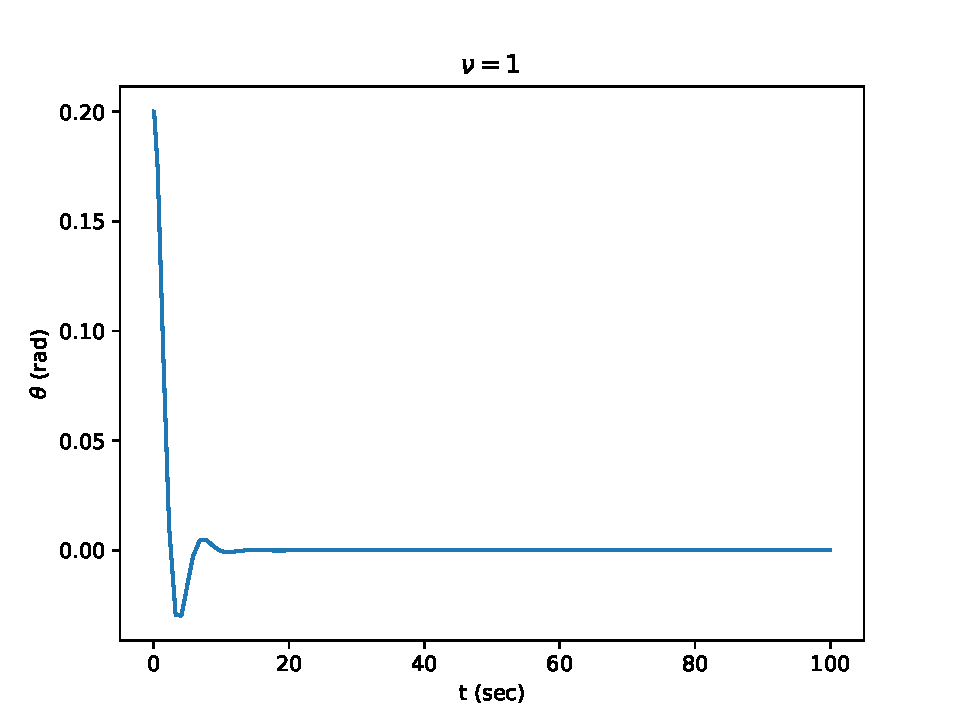
\includegraphics[width=.4\textwidth]{../figs/q1_v_1.pdf}
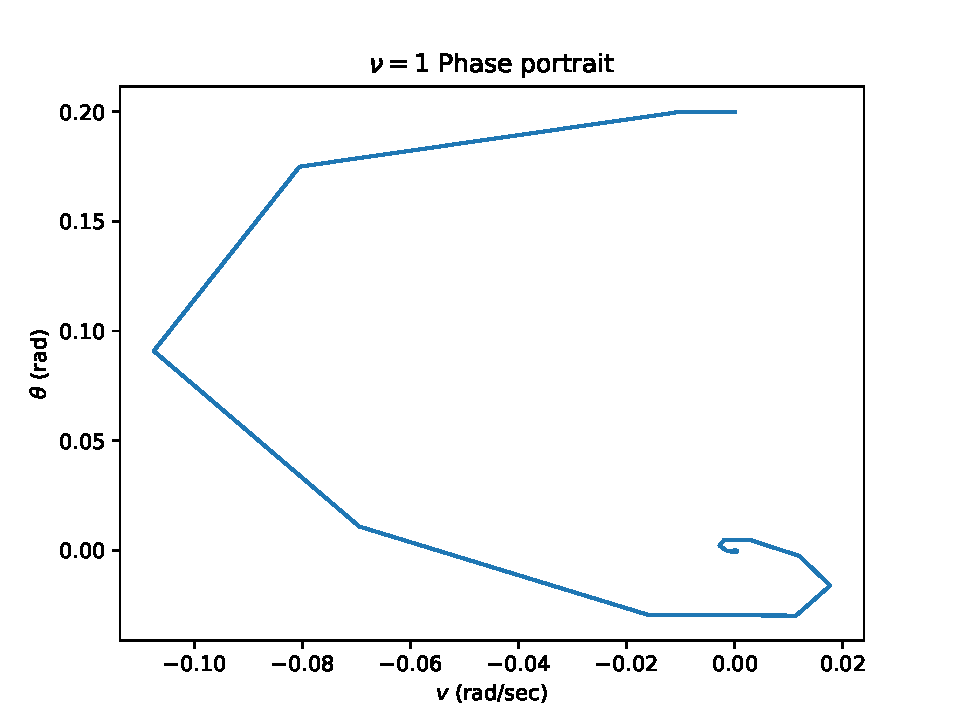
\includegraphics[width=.4\textwidth]{../figs/q1_v_1_phase.pdf}
\end{center}
\begin{center}
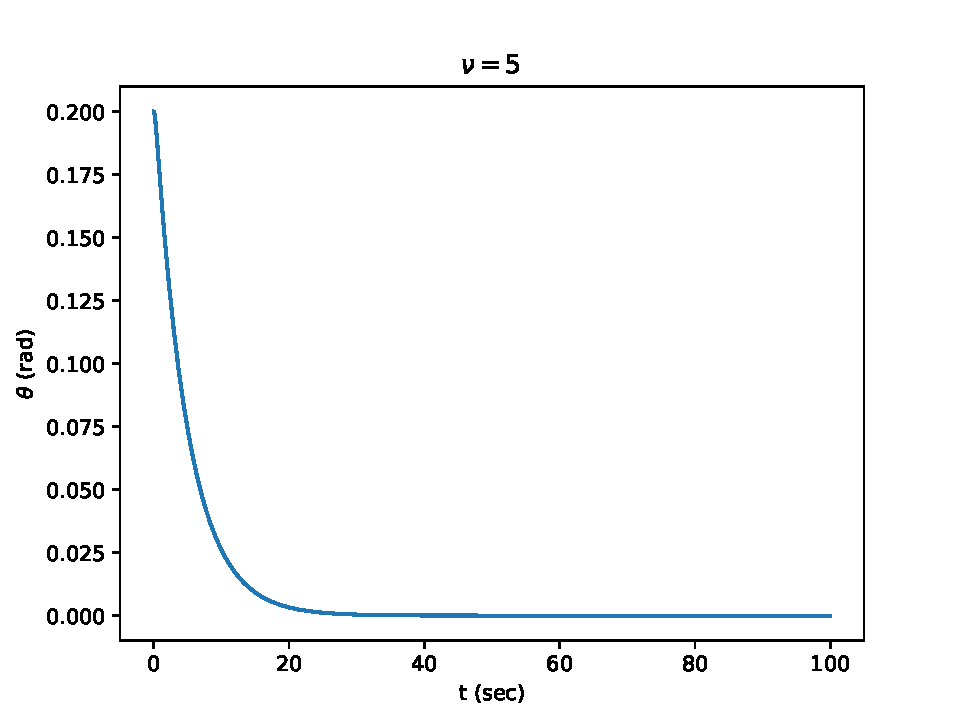
\includegraphics[width=.4\textwidth]{../figs/q1_v_5.pdf}
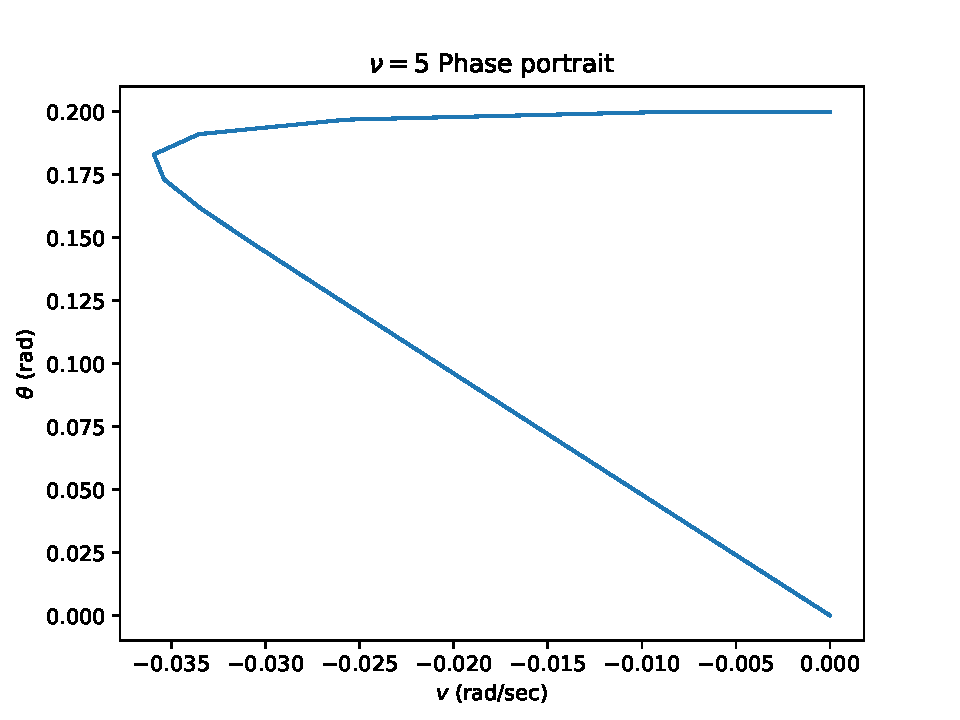
\includegraphics[width=.4\textwidth]{../figs/q1_v_5_phase.pdf}
\end{center}
\begin{center}
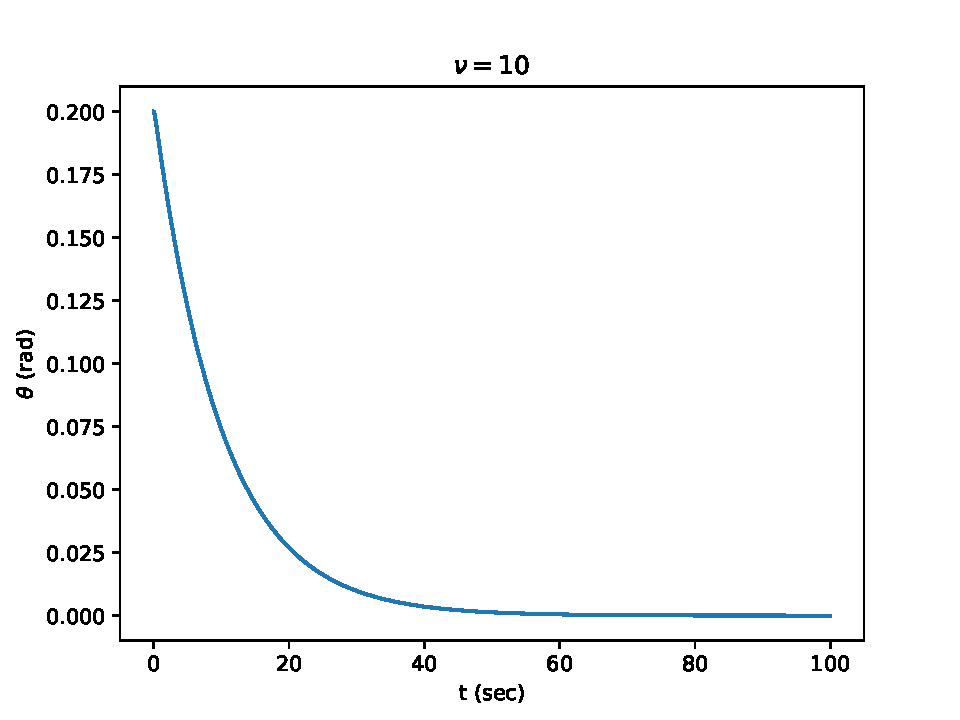
\includegraphics[width=.4\textwidth]{../figs/q1_v_10.pdf}
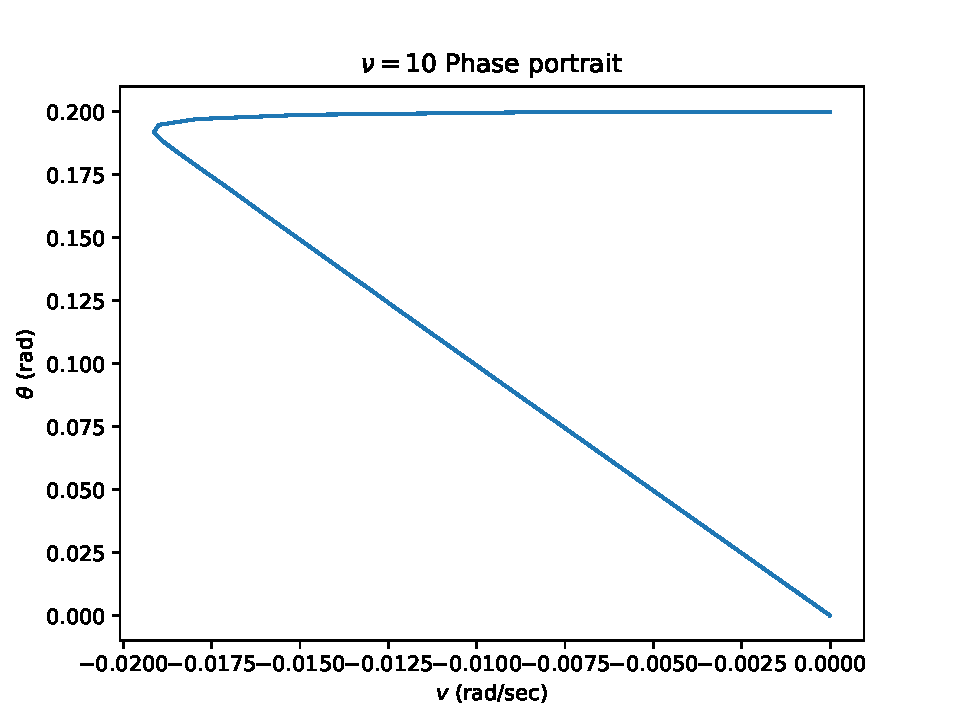
\includegraphics[width=.4\textwidth]{../figs/q1_v_10_phase.pdf}
\end{center}
\newpage
\noindent \Large{Question 2}
\\ \\
\noindent \normalsize{Please see \texttt{q2.py} in the \texttt{code} folder for relevant code for Q2.}
\\ \\
Though dense, we note that the leftmost picture pertains to a wrapped motion of $\theta$, the middle picture denotes an unwrapped photo of motion and the rightmost picture denotes athe phase portrait. From here we can see that $A=0.5$ has stable motion and is not chaotic. Given enough periods, it will stabilize to a constant periodic motion (as seen as the limits of the unwrapped version being identical to the wrapped version). However, for $A=1.2$, we can see that it resembles chaotic motion. For one, the motion overshoots the limits as we can see from the unwrapped and wrapped versions of motion. We can also make out multiple ``attractors'' from the phase portrait.
\begin{center}
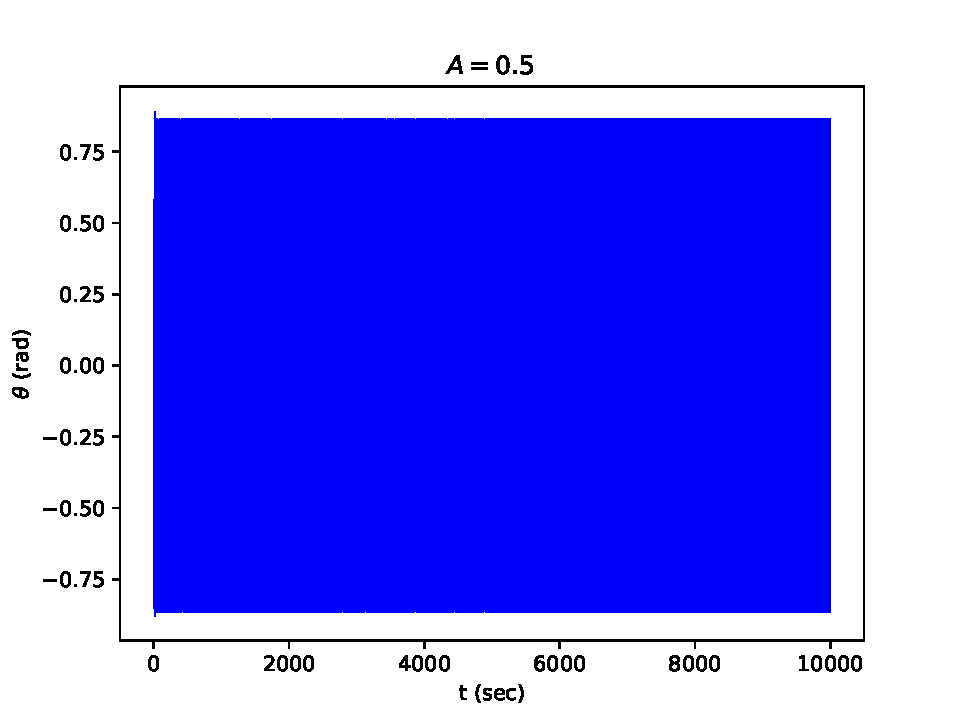
\includegraphics[width=.3\textwidth]{../figs/q2_A_05.pdf}
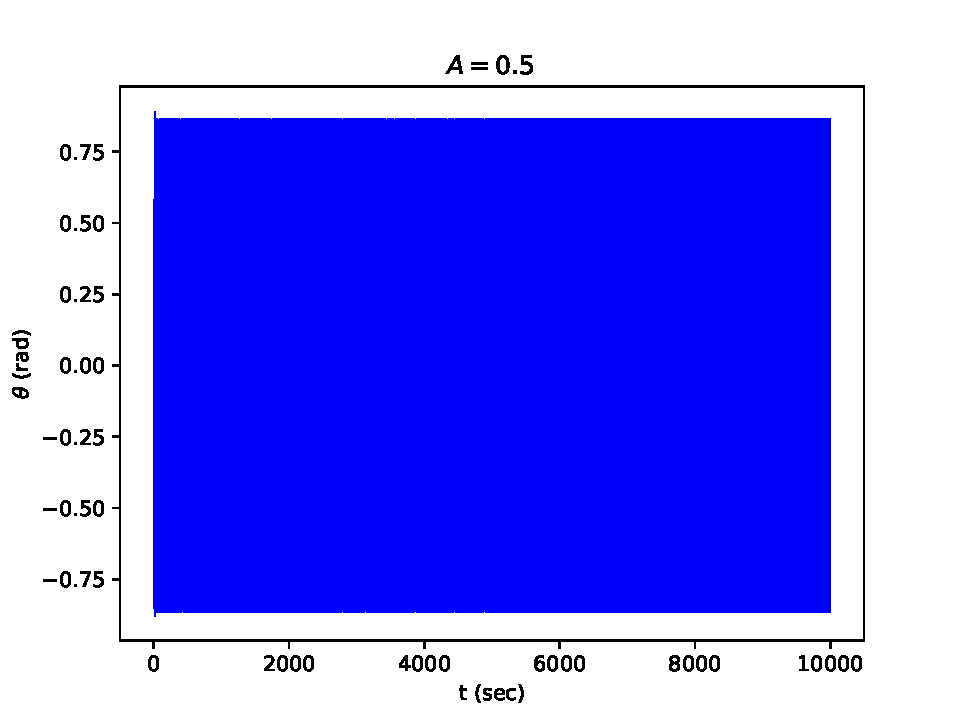
\includegraphics[width=.3\textwidth]{../figs/q2_A_05_no_wrap.pdf}
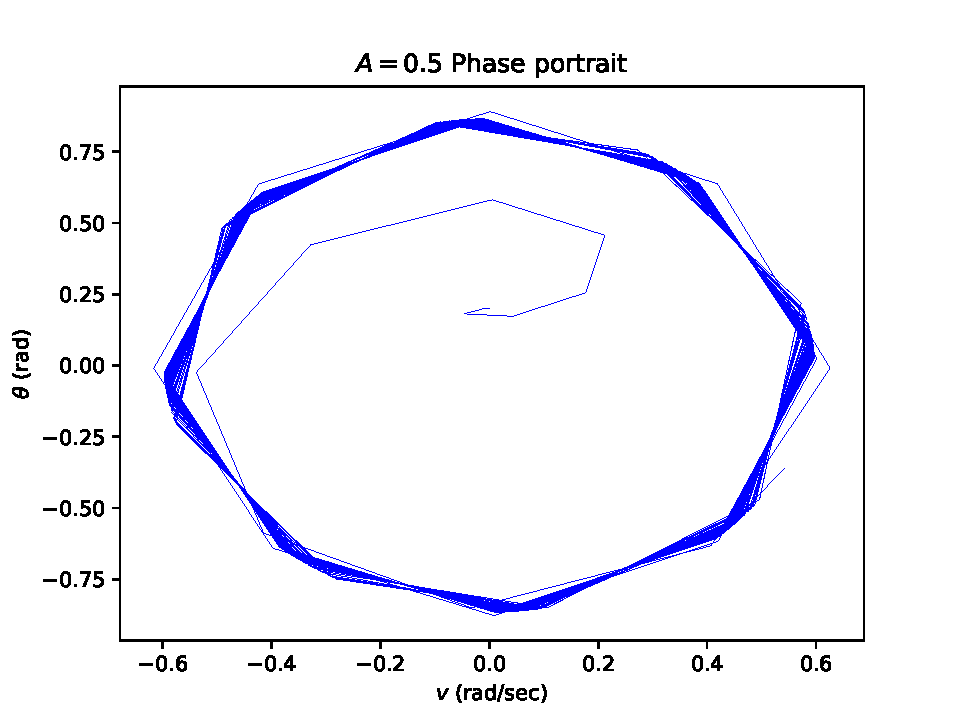
\includegraphics[width=.3\textwidth]{../figs/q2_A_05_phase.pdf}
\end{center}

\begin{center}
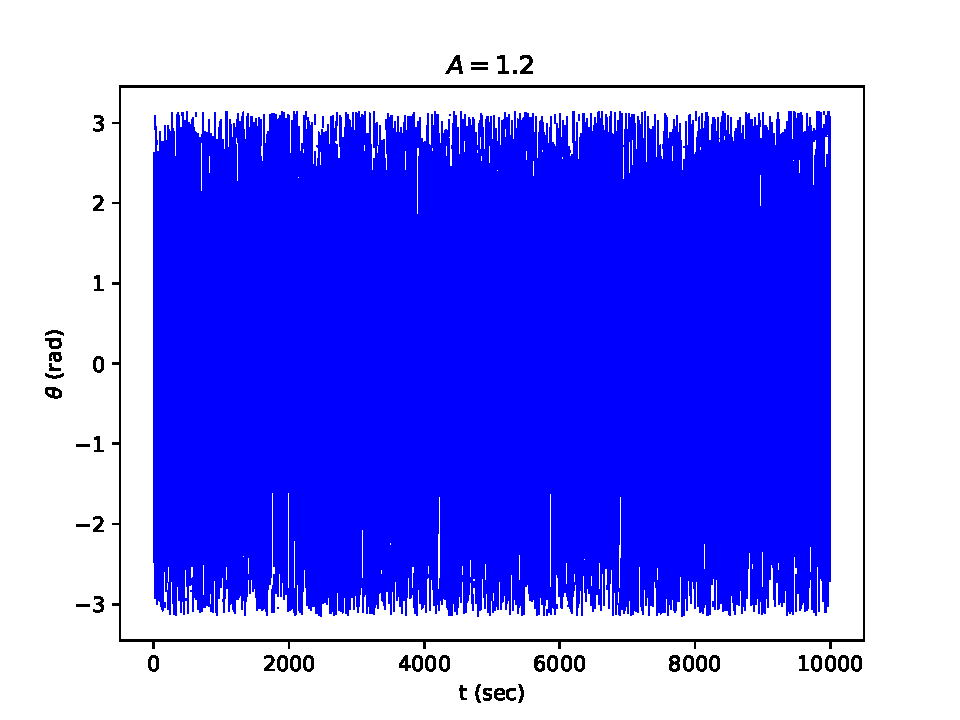
\includegraphics[width=.3\textwidth]{../figs/q2_A_12.pdf}
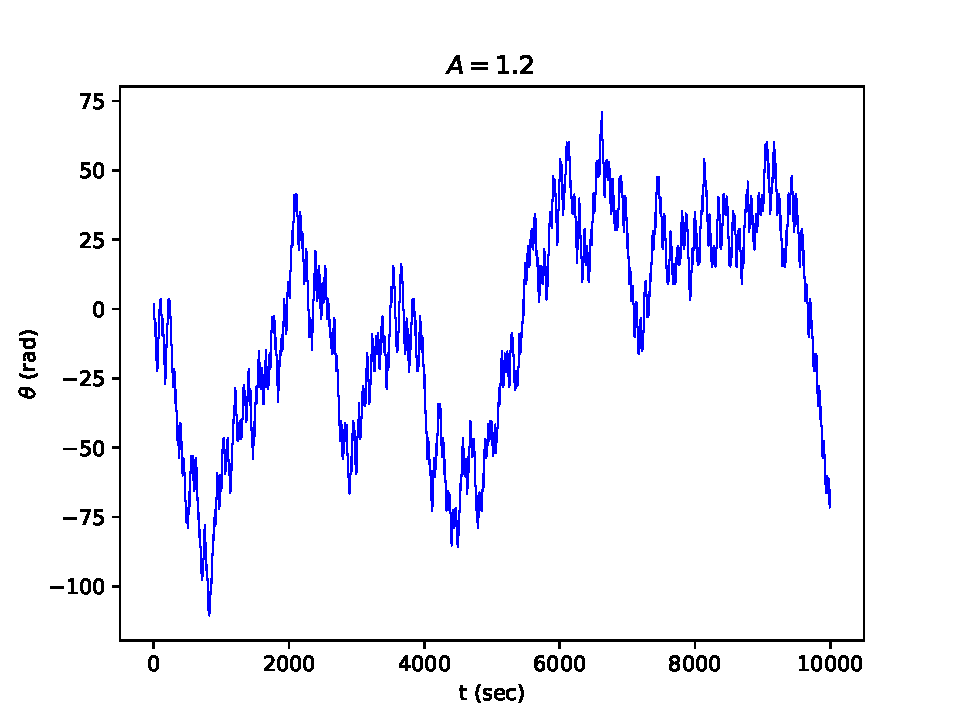
\includegraphics[width=.3\textwidth]{../figs/q2_A_12_no_wrap.pdf}
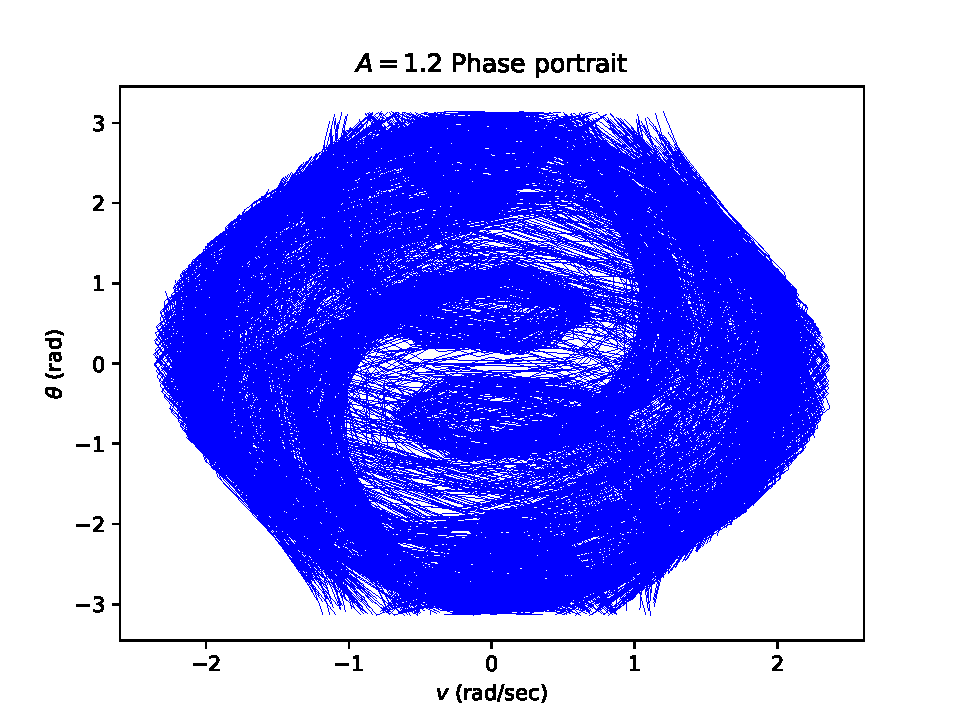
\includegraphics[width=.3\textwidth]{../figs/q2_A_12_phase.pdf}
\end{center}
\noindent \Large{Question 3}
\\ \\
\noindent \normalsize{Please see \texttt{q3.py} in the \texttt{code} folder for relevant code for Q3.}
\\ \\
The same layout as last question. Since we did the \texttt{RK45} method (from python which is analogous of \texttt{ode45}), we adjusted the \texttt{relTol}. We made ours \texttt{1e-13} to smoothen out the phase portrait (we can see that the phase portraits made now are smoother than those of previous questions.) While differing amplitudes of the driving force, we can see that as we increase A, we start with a stable single attractor, then at around $A=1$, we get a separatix state and we transition to still a single attractor, but one that overshoots the domain of [$-\pi, \pi$] (hence the resemblance of $A=0.9$ and $A=1.4$ in $A=1.2$). As we keep increasing, we do end up with defined attractors, but they become more rare and far in between.
\begin{center}
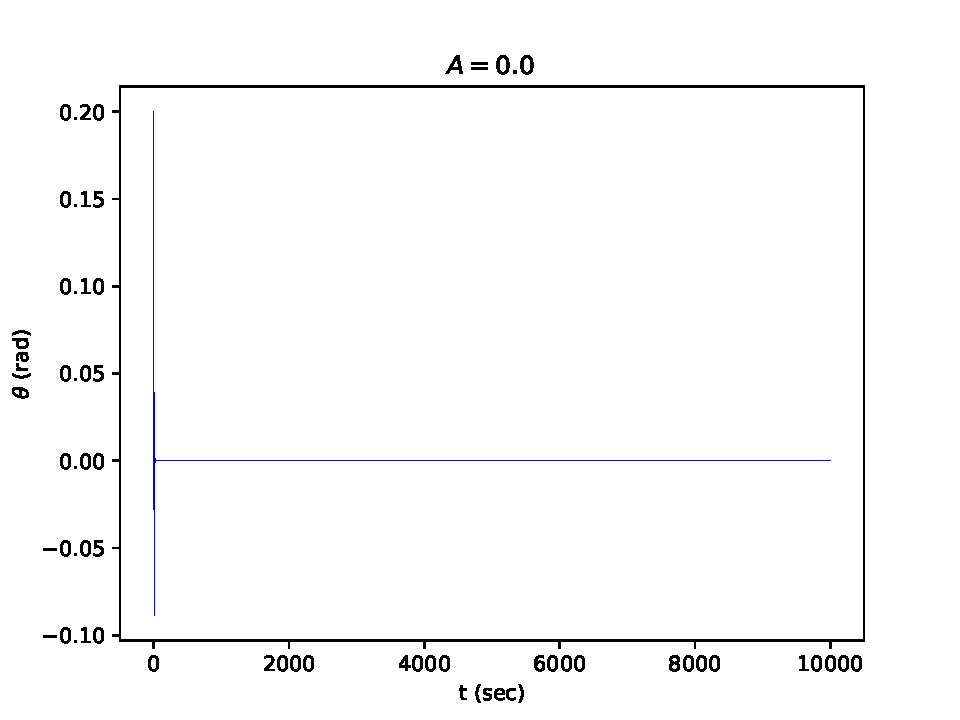
\includegraphics[width=.3\textwidth]{../figs/q3_A_00.pdf}
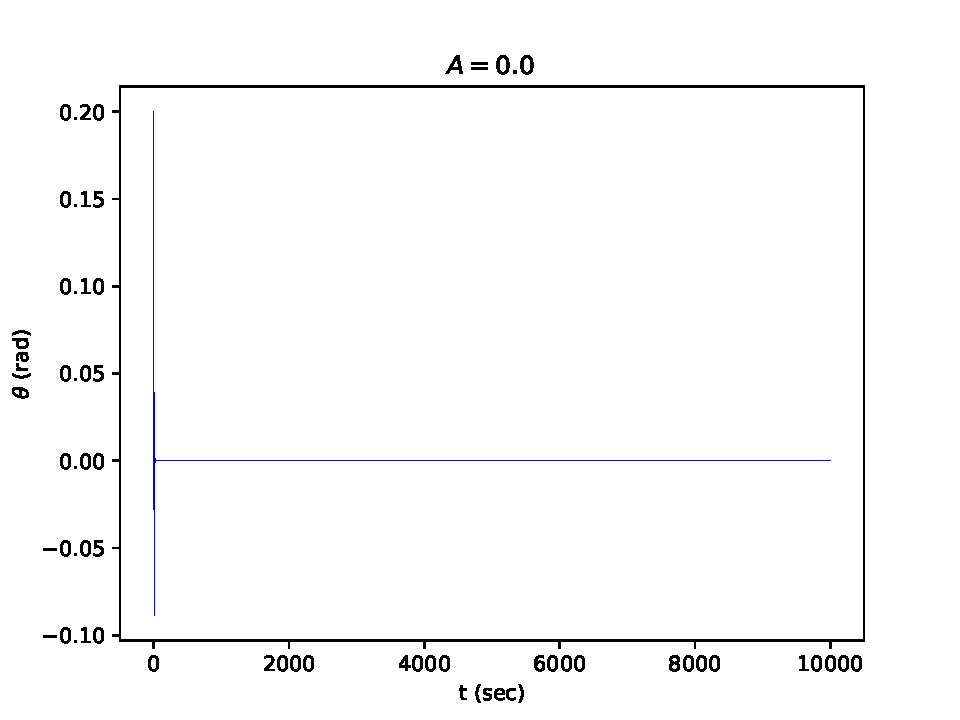
\includegraphics[width=.3\textwidth]{../figs/q3_A_00_no_wrap.pdf}
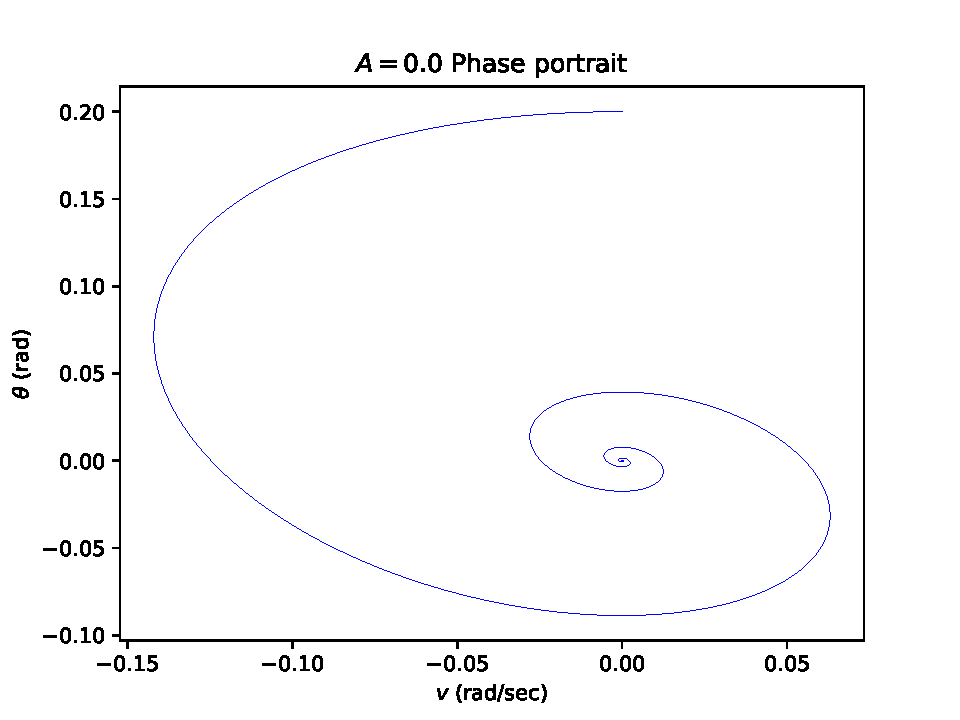
\includegraphics[width=.3\textwidth]{../figs/q3_A_00_phase.pdf}
\end{center}
\begin{center}
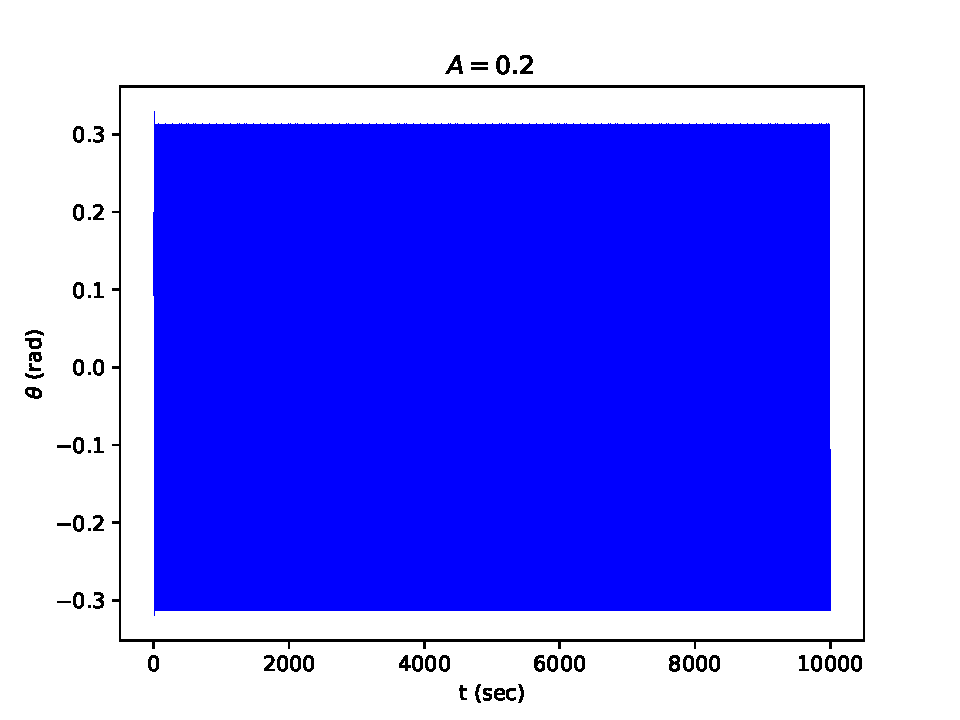
\includegraphics[width=.3\textwidth]{../figs/q3_A_02.pdf}
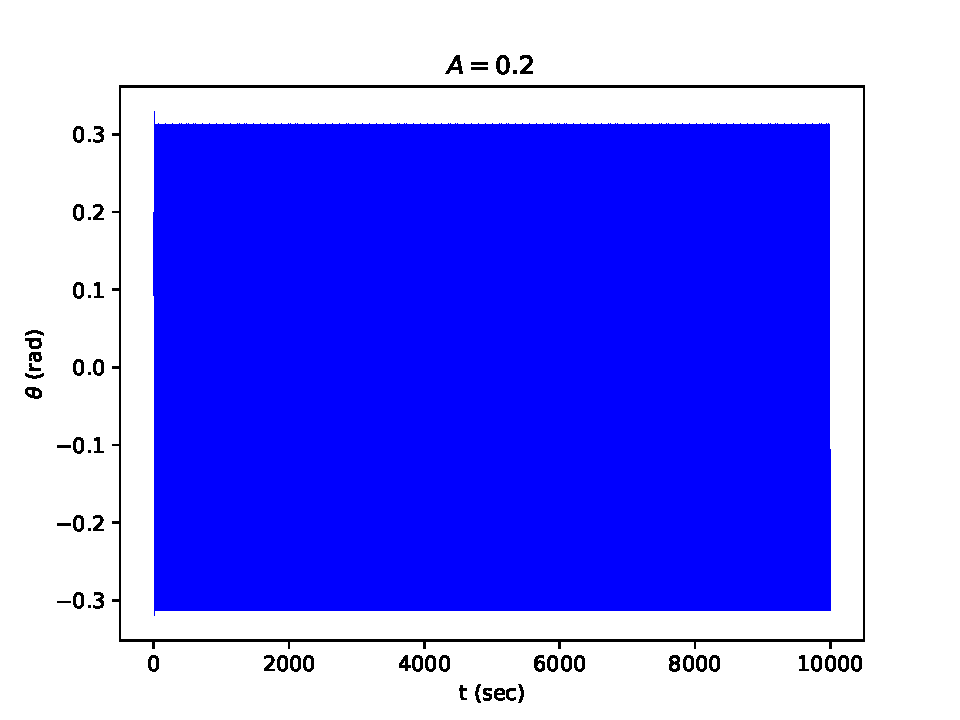
\includegraphics[width=.3\textwidth]{../figs/q3_A_02_no_wrap.pdf}
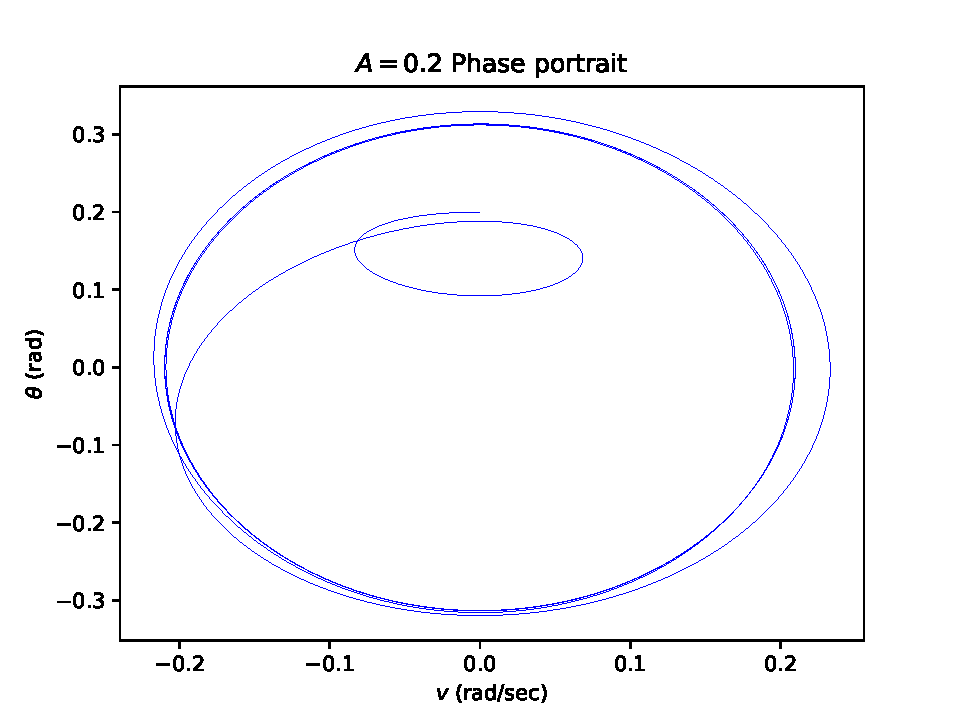
\includegraphics[width=.3\textwidth]{../figs/q3_A_02_phase.pdf}
\end{center}
\begin{center}
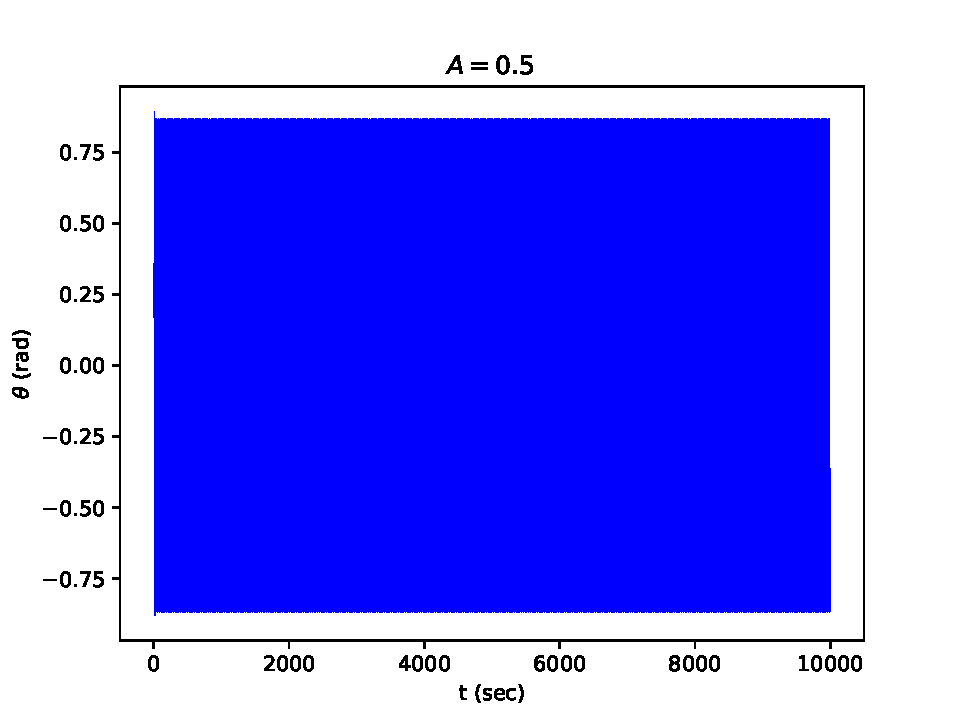
\includegraphics[width=.3\textwidth]{../figs/q3_A_05.pdf}
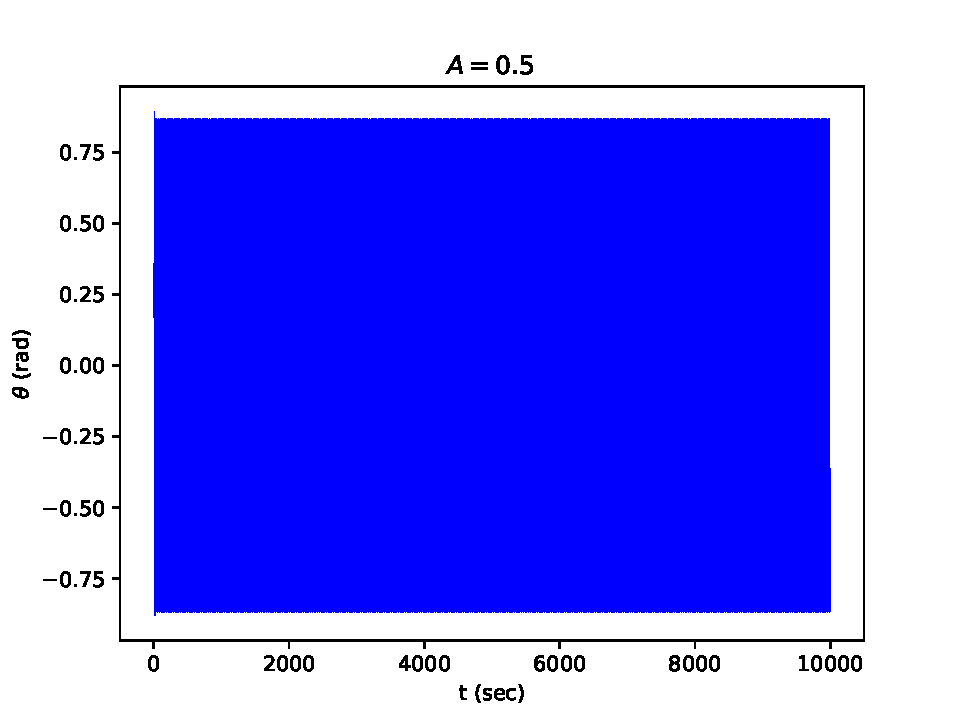
\includegraphics[width=.3\textwidth]{../figs/q3_A_05_no_wrap.pdf}
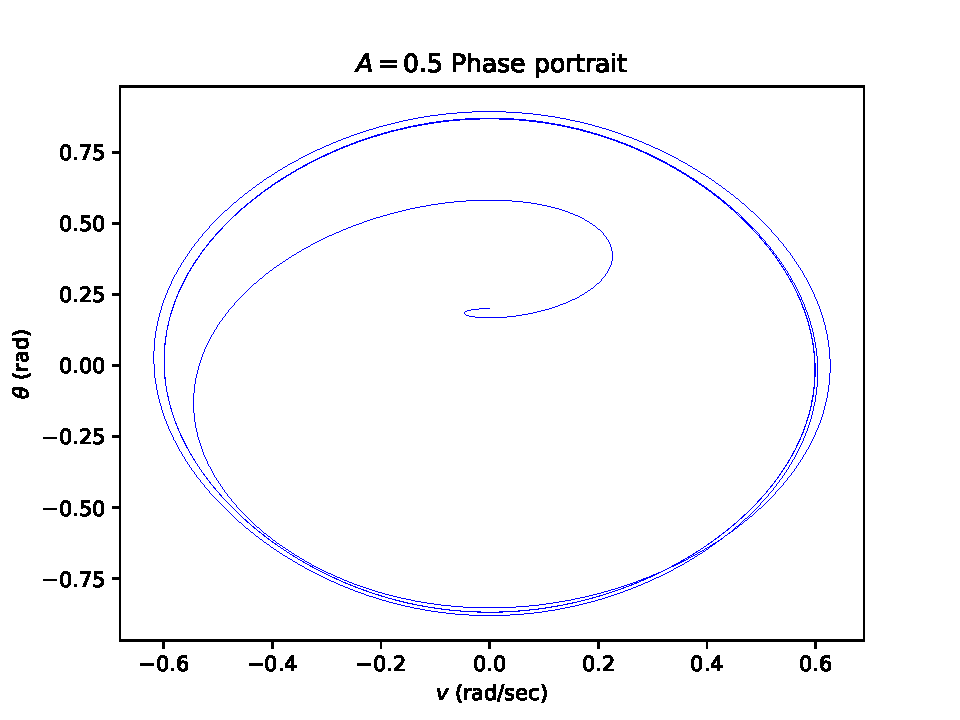
\includegraphics[width=.3\textwidth]{../figs/q3_A_05_phase.pdf}
\end{center}
\begin{center}
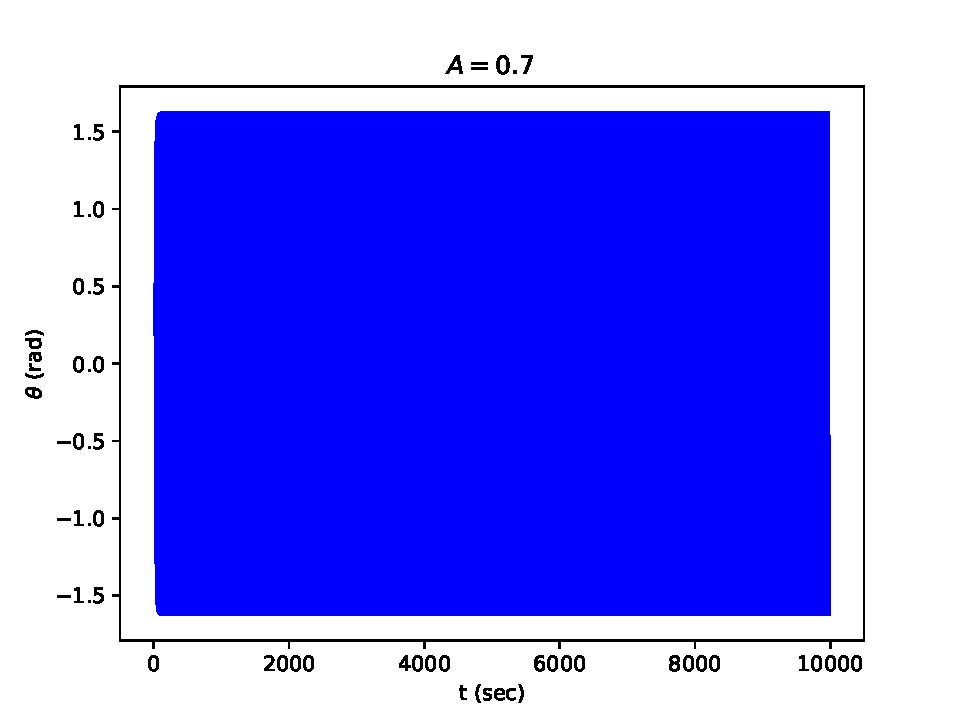
\includegraphics[width=.3\textwidth]{../figs/q3_A_07.pdf}
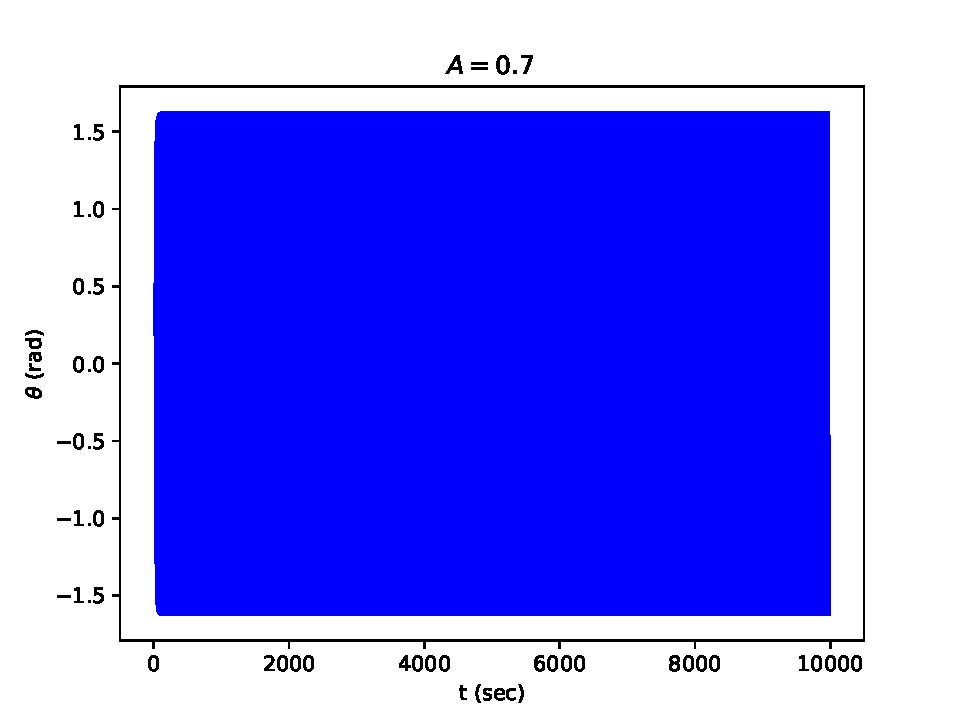
\includegraphics[width=.3\textwidth]{../figs/q3_A_07_no_wrap.pdf}
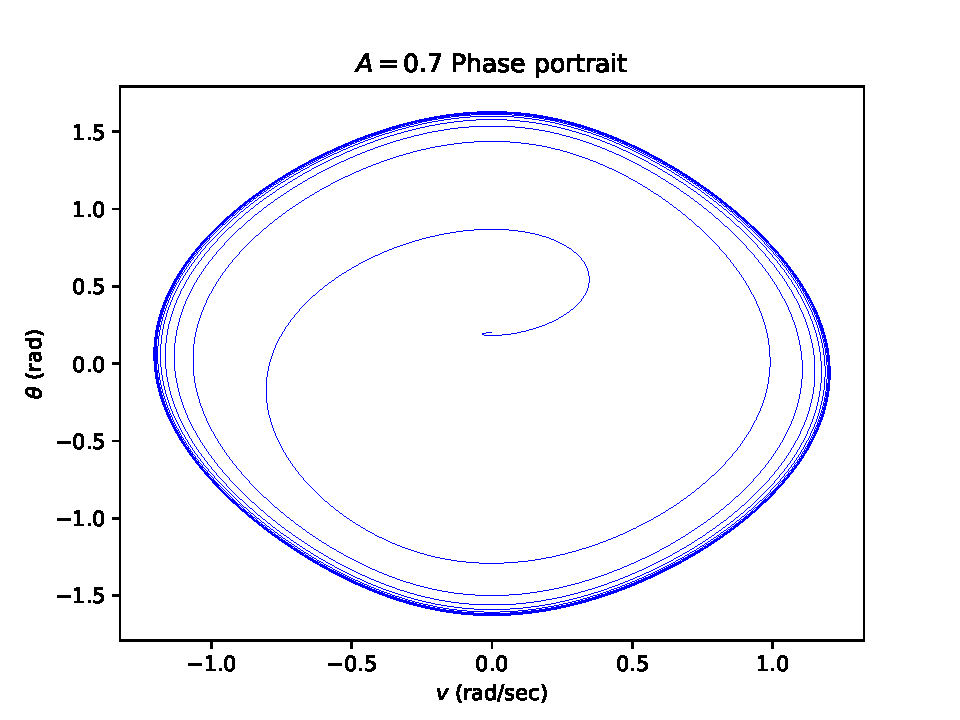
\includegraphics[width=.3\textwidth]{../figs/q3_A_07_phase.pdf}
\end{center}
\begin{center}
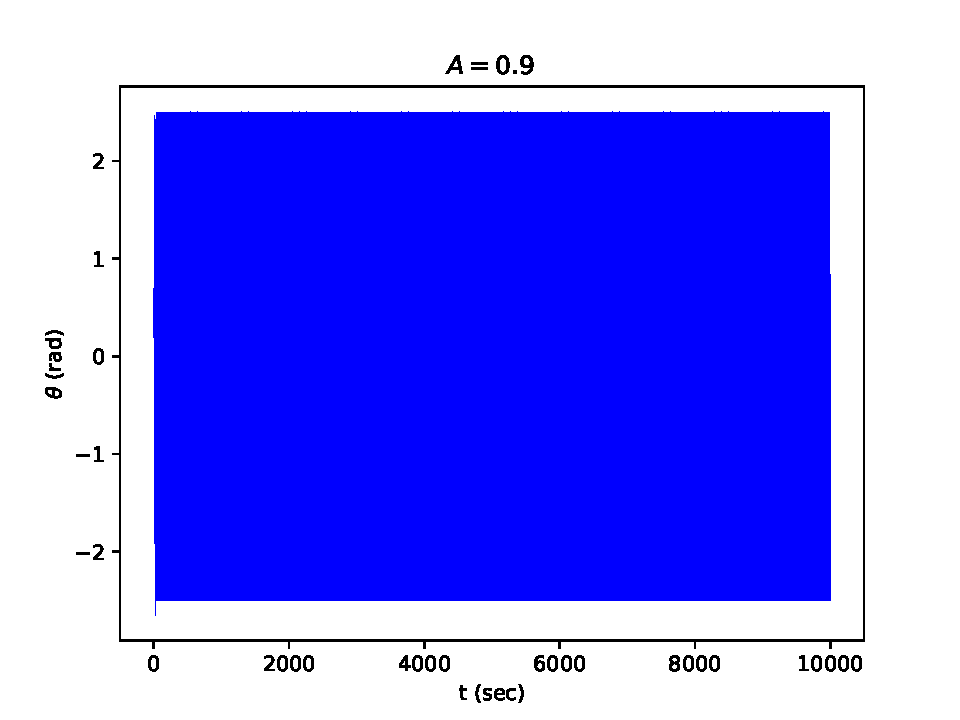
\includegraphics[width=.3\textwidth]{../figs/q3_A_09.pdf}
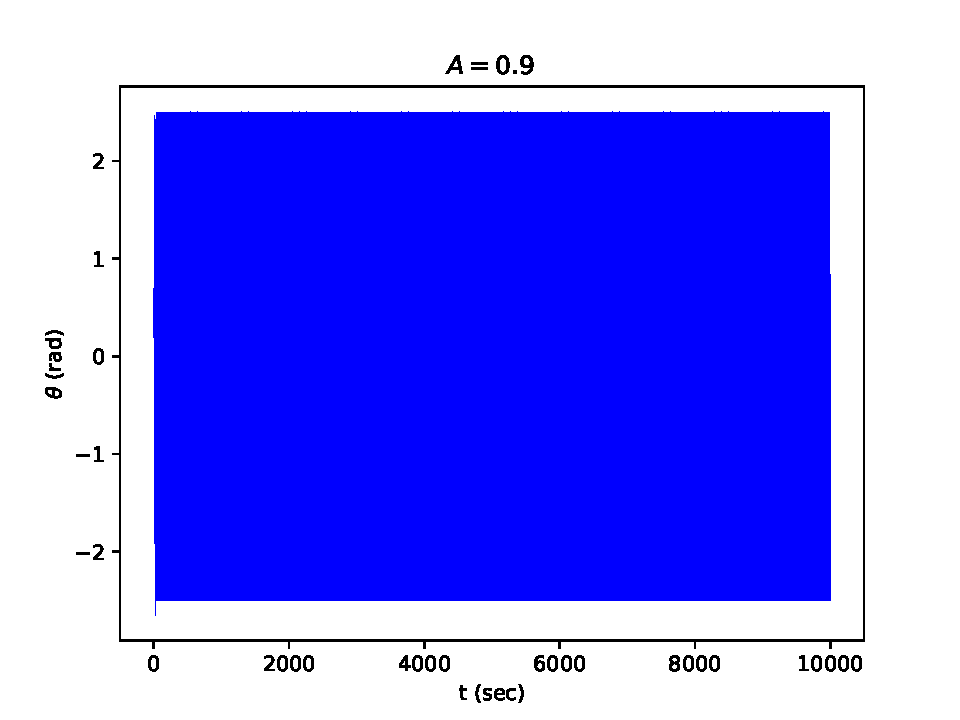
\includegraphics[width=.3\textwidth]{../figs/q3_A_09_no_wrap.pdf}
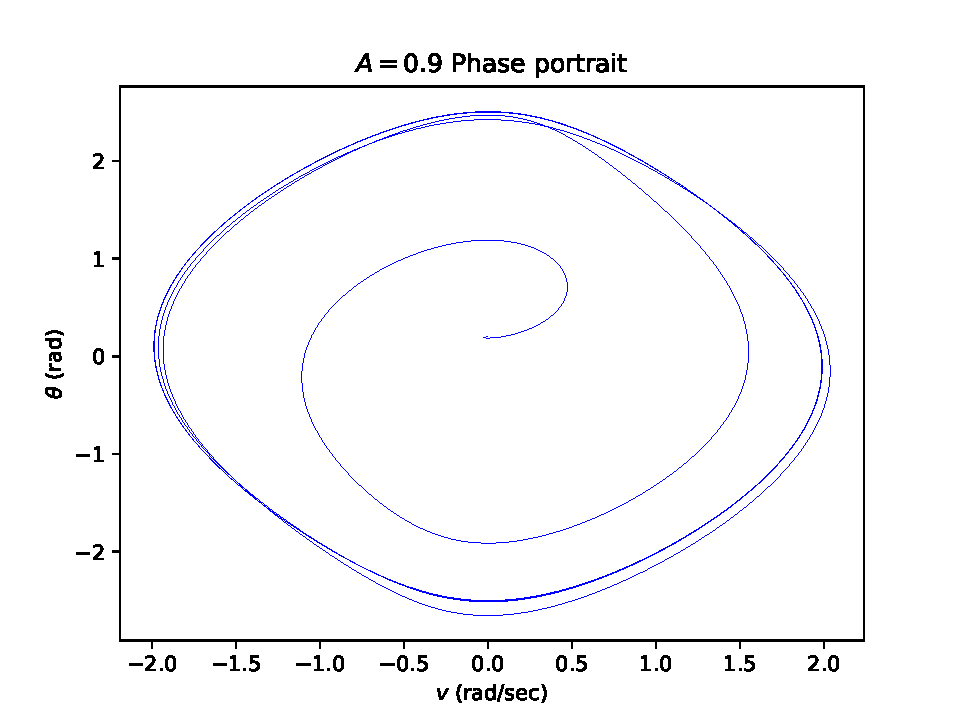
\includegraphics[width=.3\textwidth]{../figs/q3_A_09_phase.pdf}
\end{center}
\begin{center}
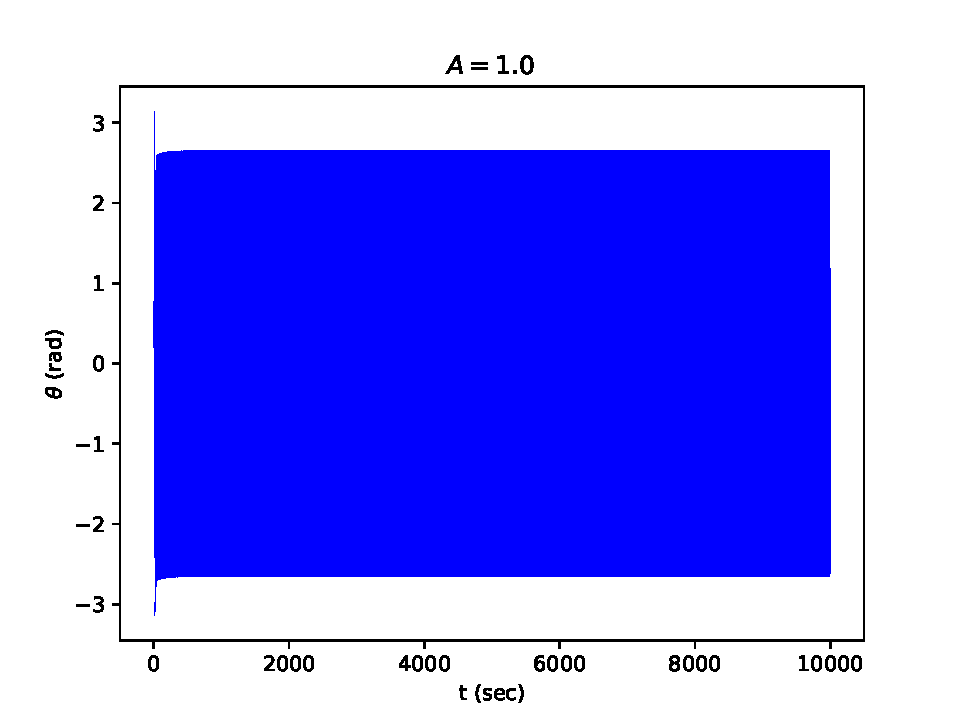
\includegraphics[width=.3\textwidth]{../figs/q3_A_10.pdf}
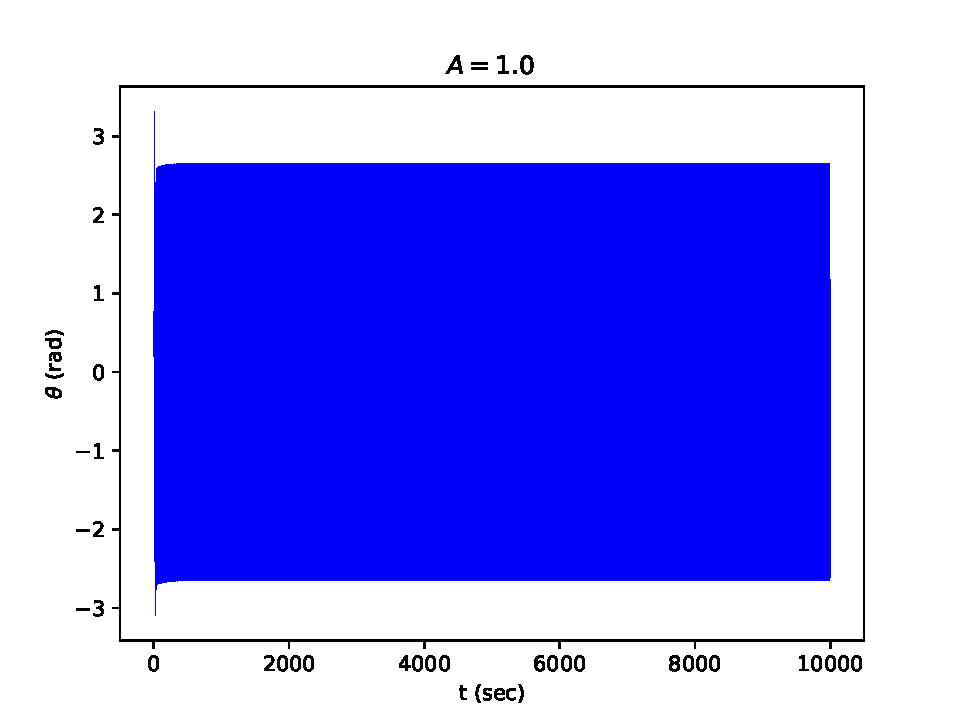
\includegraphics[width=.3\textwidth]{../figs/q3_A_10_no_wrap.pdf}
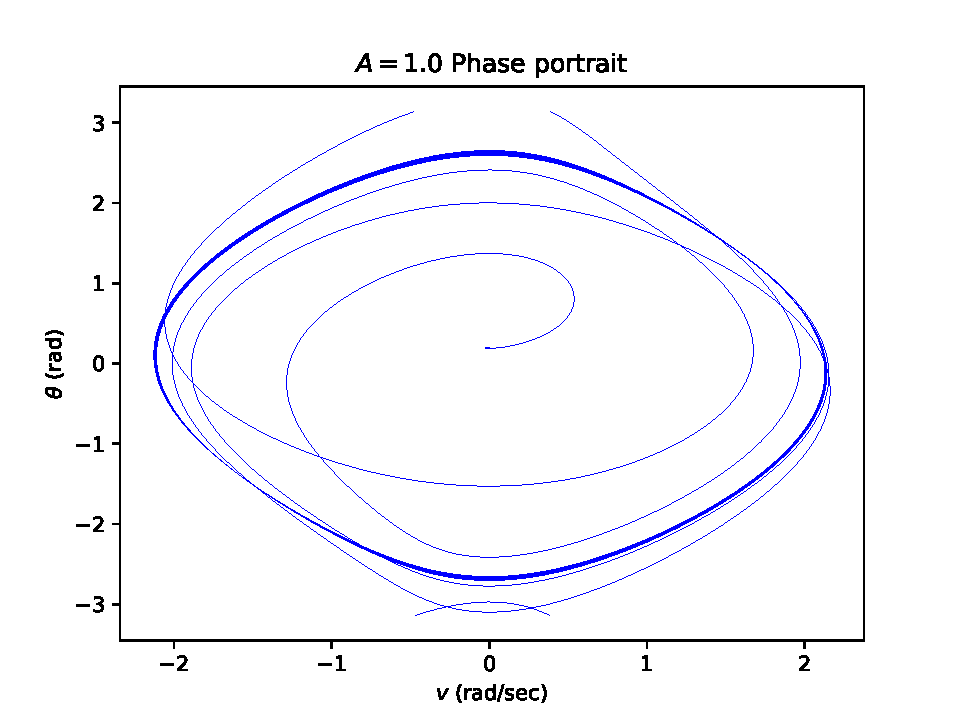
\includegraphics[width=.3\textwidth]{../figs/q3_A_10_phase.pdf}
\end{center}
\begin{center}
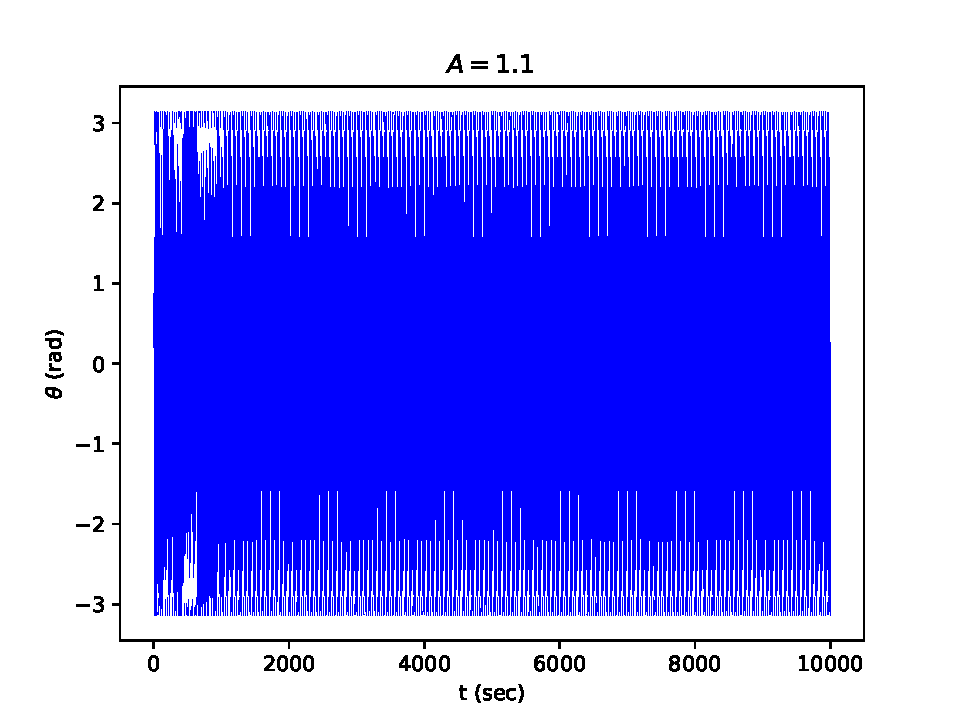
\includegraphics[width=.3\textwidth]{../figs/q3_A_11.pdf}
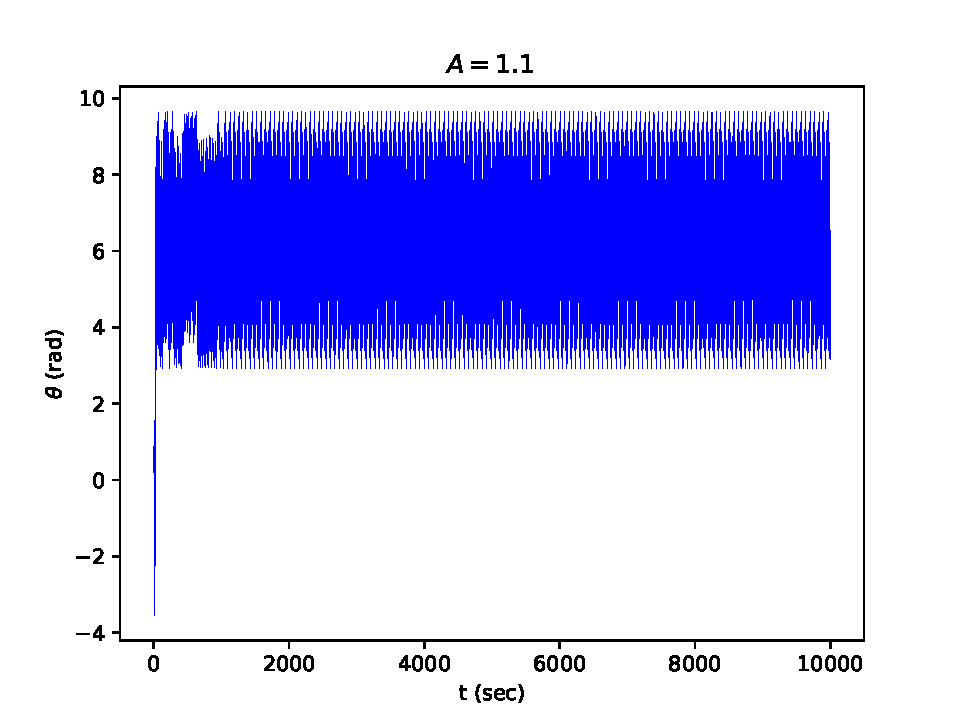
\includegraphics[width=.3\textwidth]{../figs/q3_A_11_no_wrap.pdf}
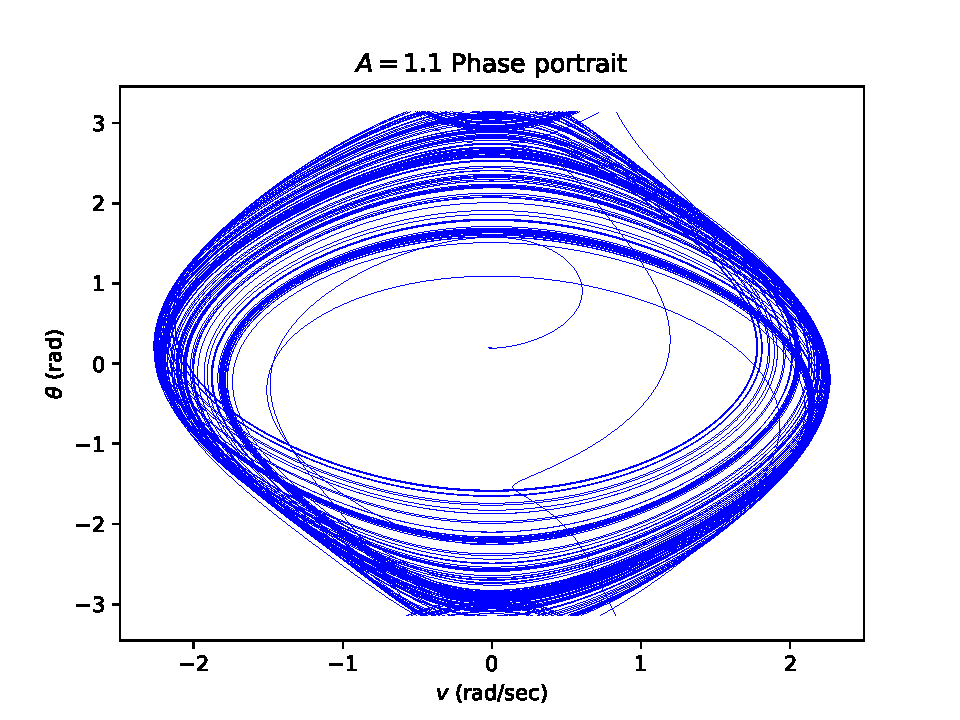
\includegraphics[width=.3\textwidth]{../figs/q3_A_11_phase.pdf}
\end{center}
\begin{center}
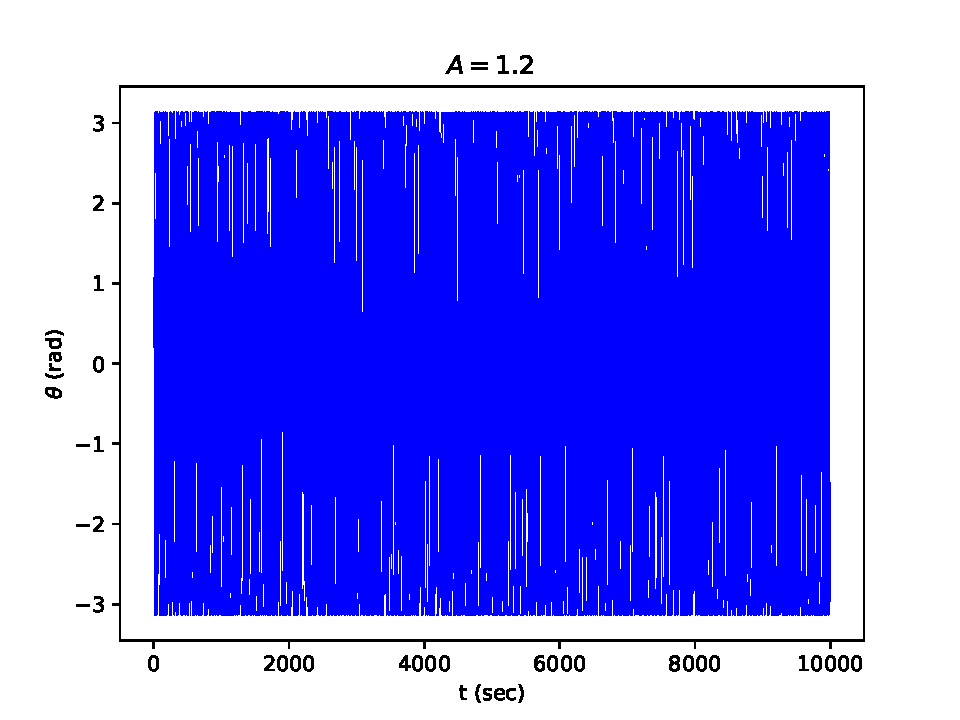
\includegraphics[width=.3\textwidth]{../figs/q3_A_12.pdf}
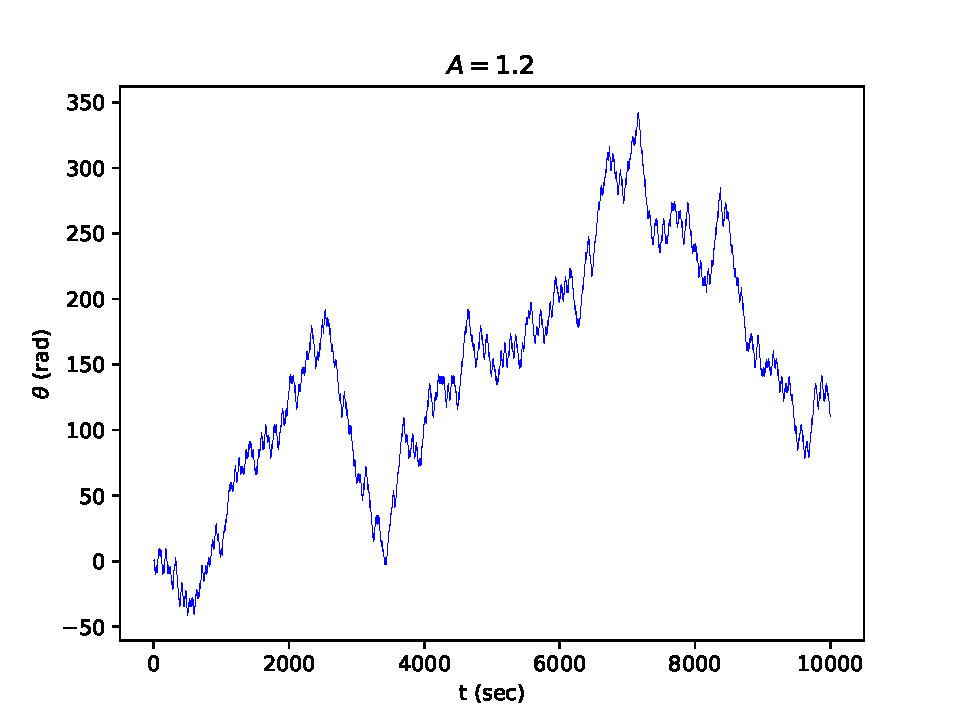
\includegraphics[width=.3\textwidth]{../figs/q3_A_12_no_wrap.pdf}
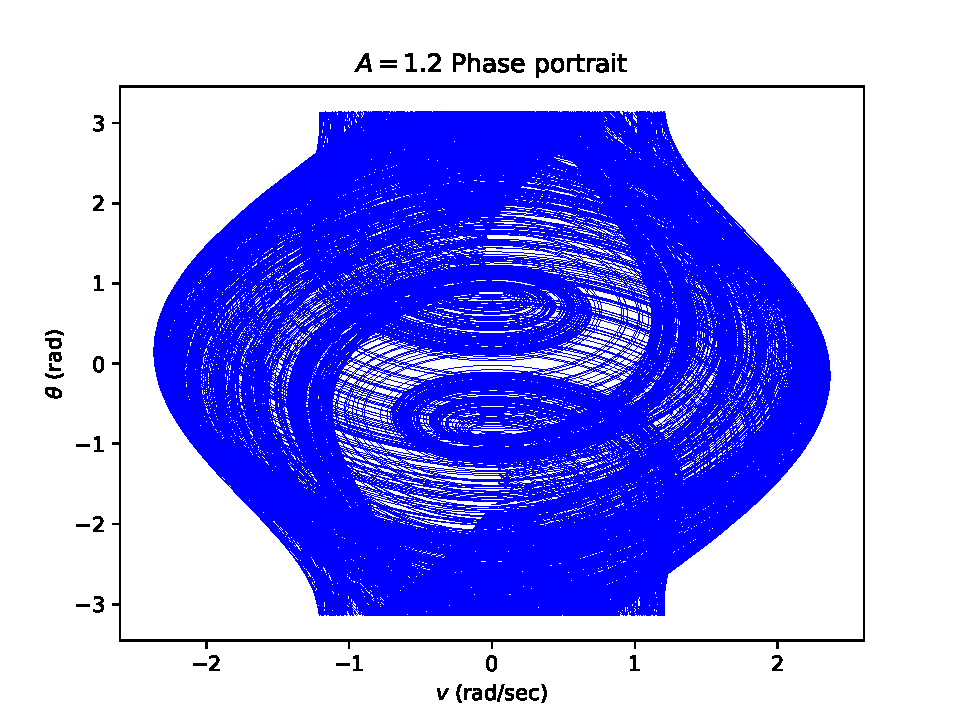
\includegraphics[width=.3\textwidth]{../figs/q3_A_12_phase.pdf}
\end{center}
\begin{center}
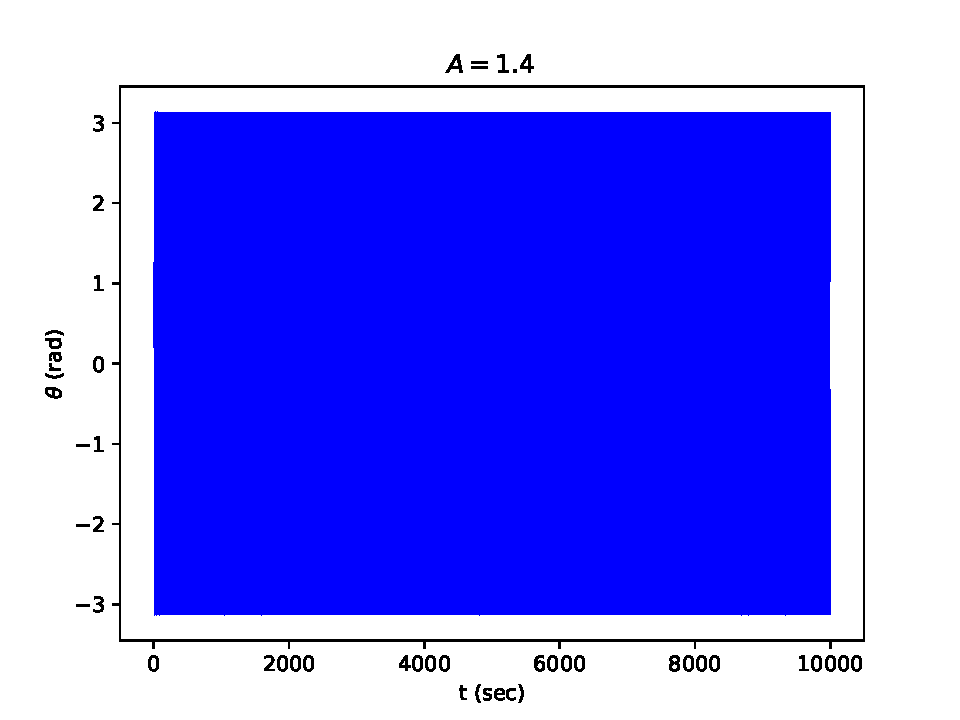
\includegraphics[width=.3\textwidth]{../figs/q3_A_14.pdf}
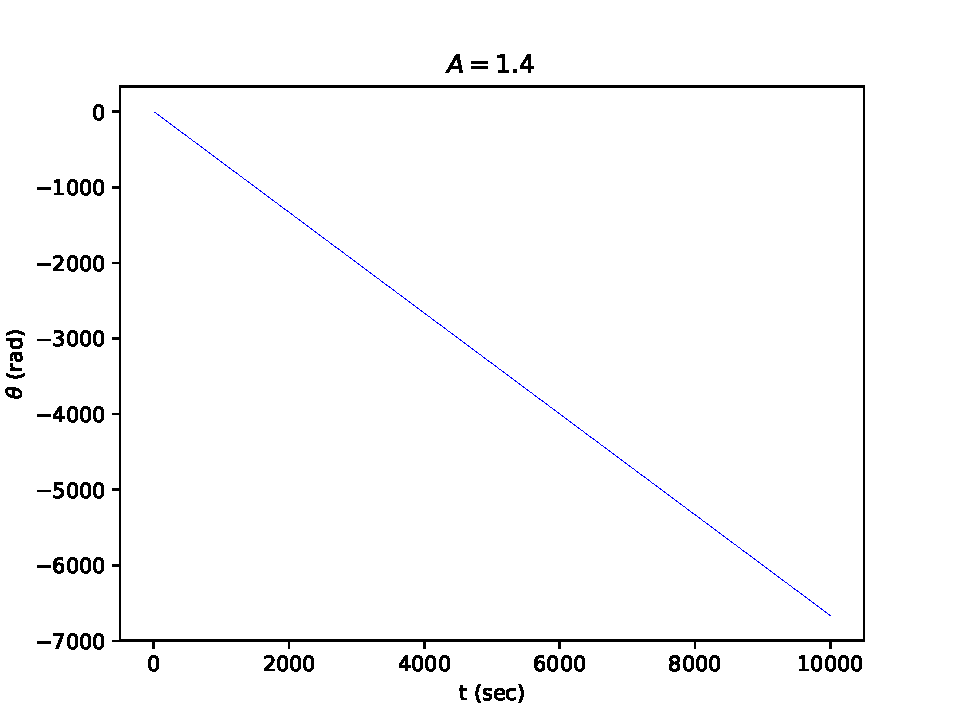
\includegraphics[width=.3\textwidth]{../figs/q3_A_14_no_wrap.pdf}
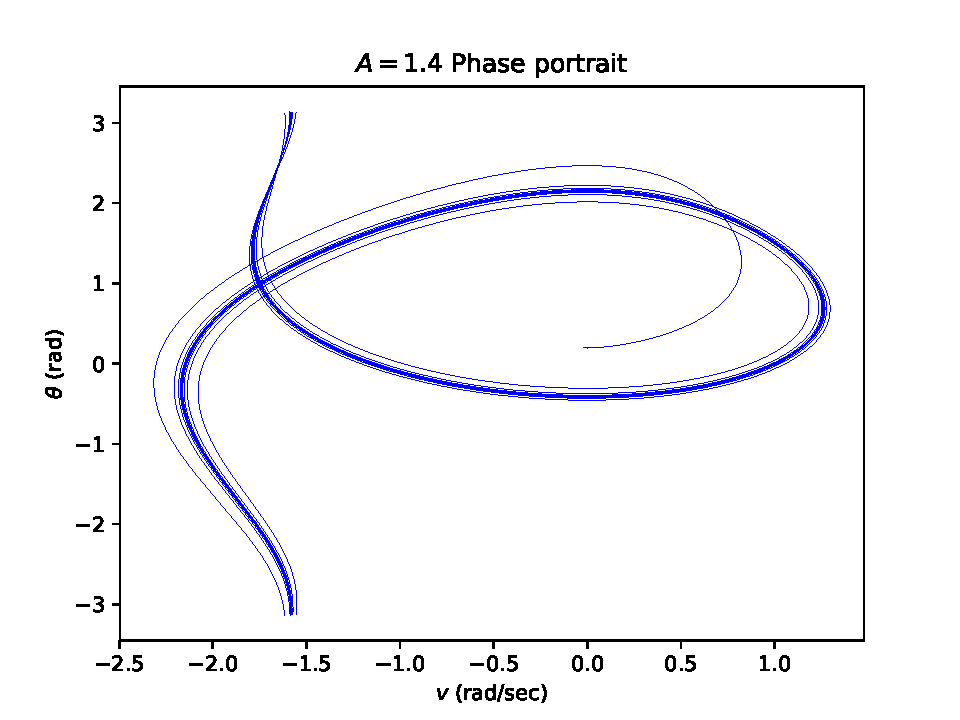
\includegraphics[width=.3\textwidth]{../figs/q3_A_14_phase.pdf}
\end{center}
\begin{center}
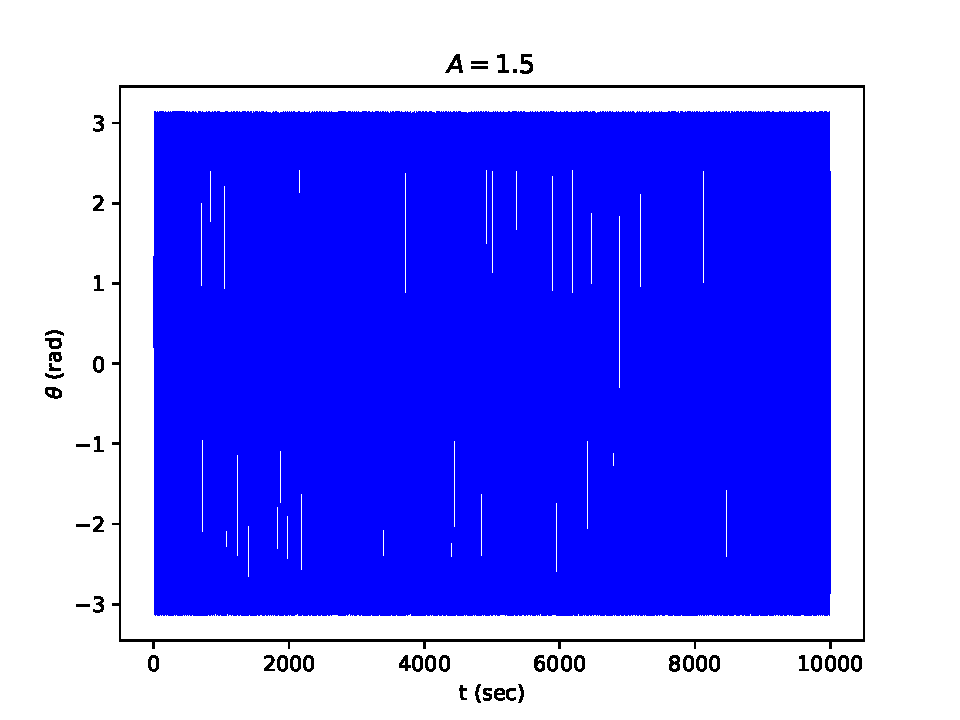
\includegraphics[width=.3\textwidth]{../figs/q3_A_15.pdf}
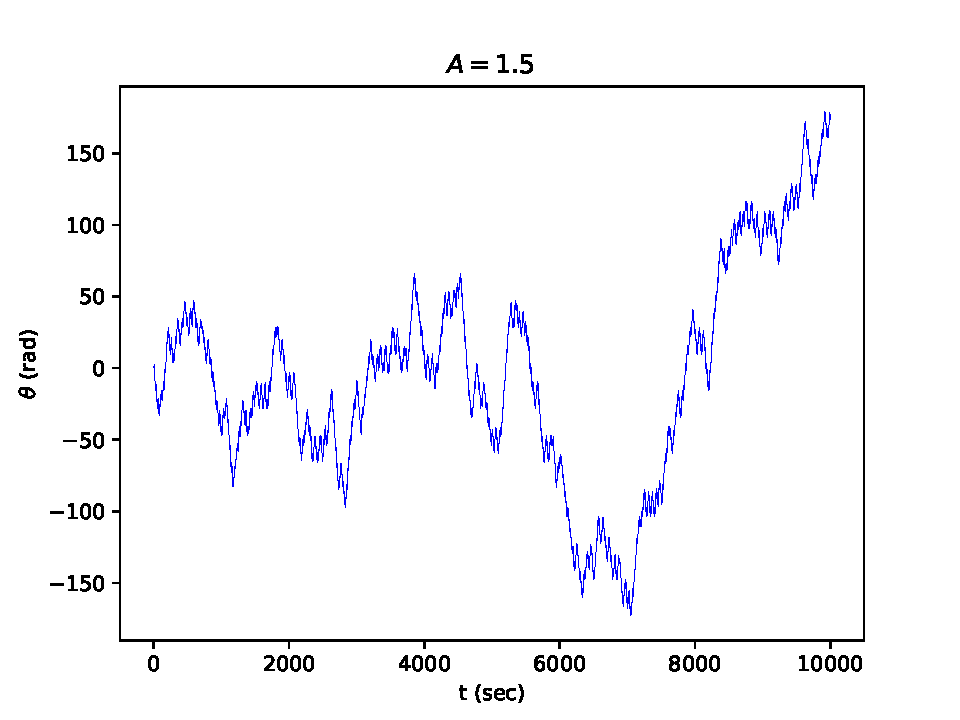
\includegraphics[width=.3\textwidth]{../figs/q3_A_15_no_wrap.pdf}
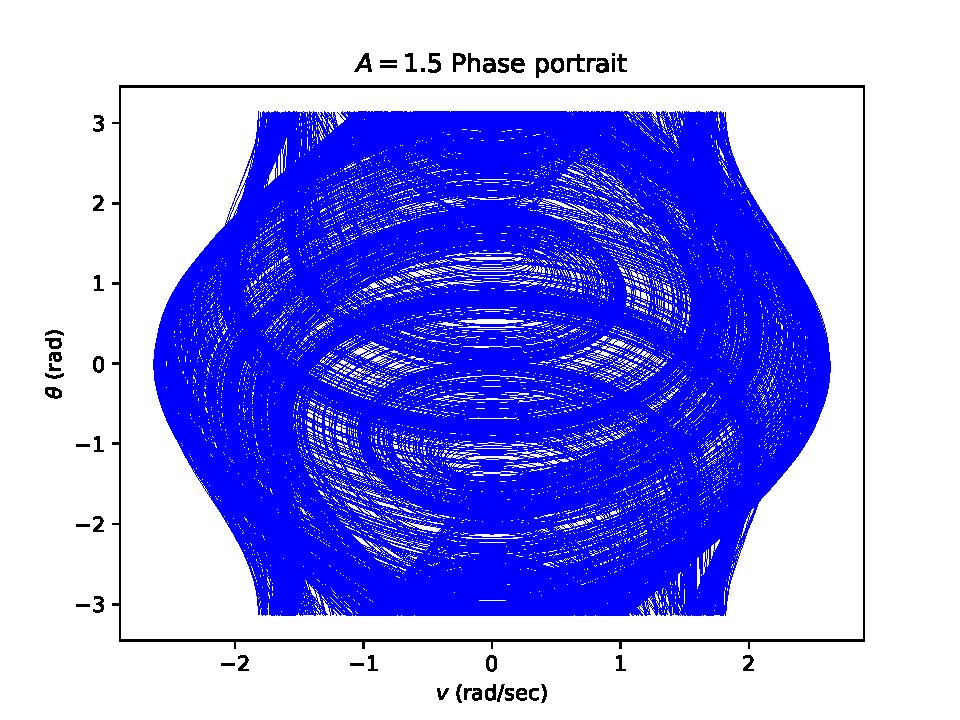
\includegraphics[width=.3\textwidth]{../figs/q3_A_15_phase.pdf}
\end{center}
\begin{center}
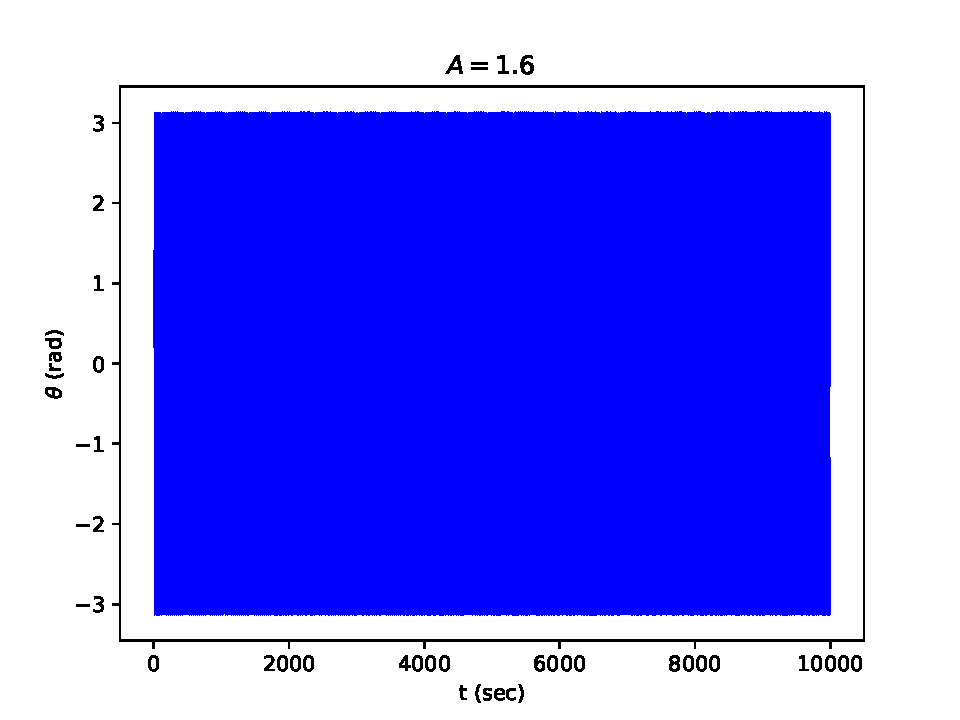
\includegraphics[width=.3\textwidth]{../figs/q3_A_16.pdf}
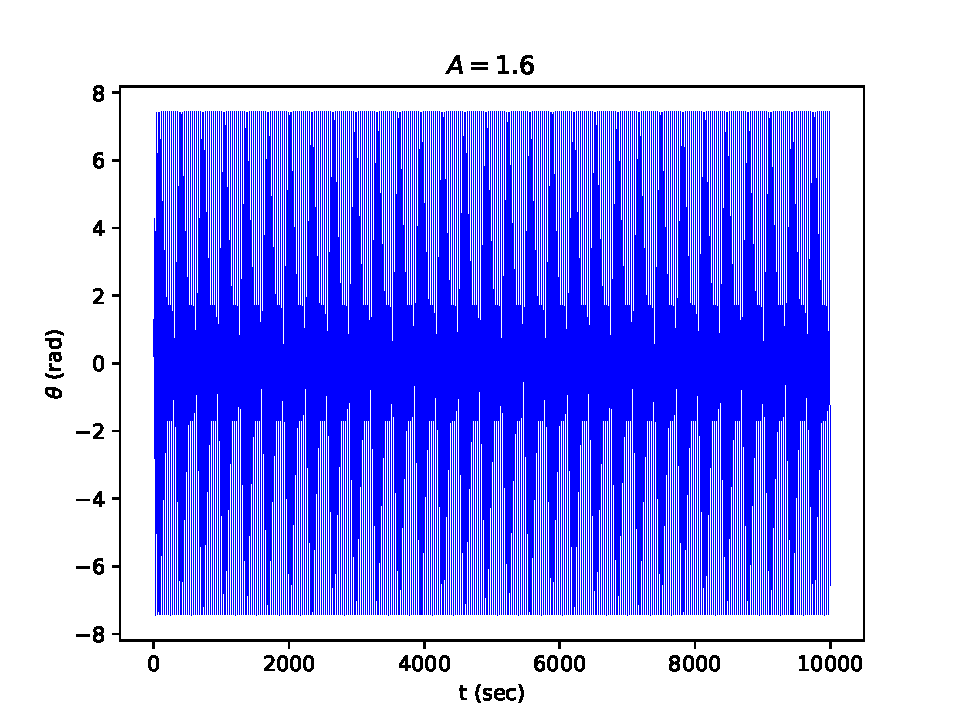
\includegraphics[width=.3\textwidth]{../figs/q3_A_16_no_wrap.pdf}
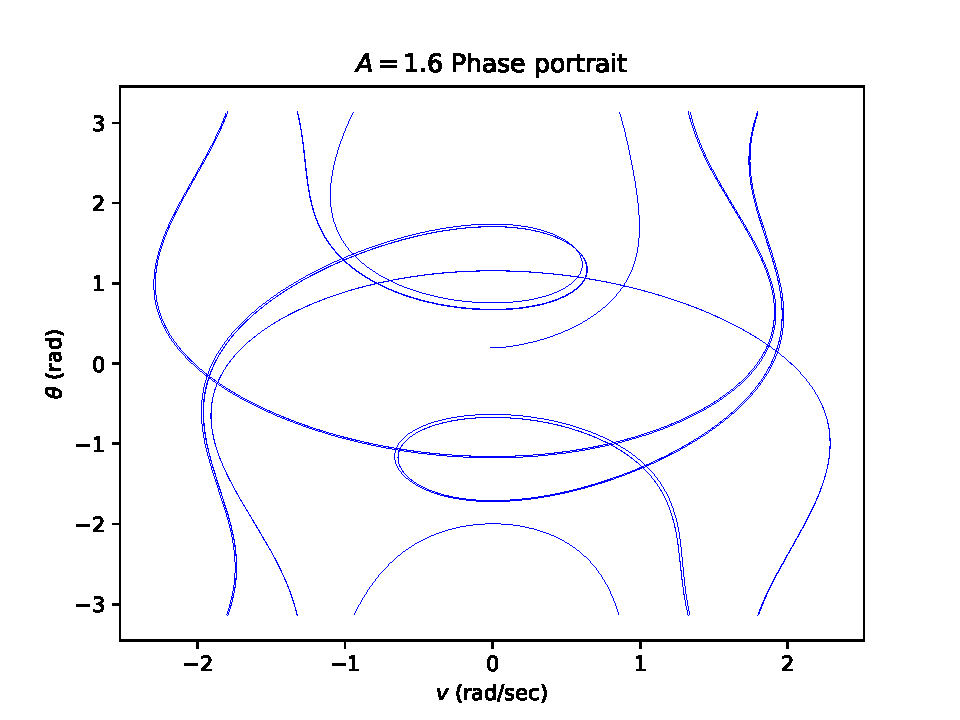
\includegraphics[width=.3\textwidth]{../figs/q3_A_16_phase.pdf}
\end{center}
\newpage
\noindent \Large{Question 4}
\\ \\
\noindent \normalsize{Please see \texttt{q4.py} in the \texttt{code} folder for relevant code for Q4.}
\\ \\
Similar to the plots at the latter part of Q3, we can see that a well-define attractor at arround $A=1.35$. As we veer away from 1.35, we get increasingly more chaotic states.
\begin{center}
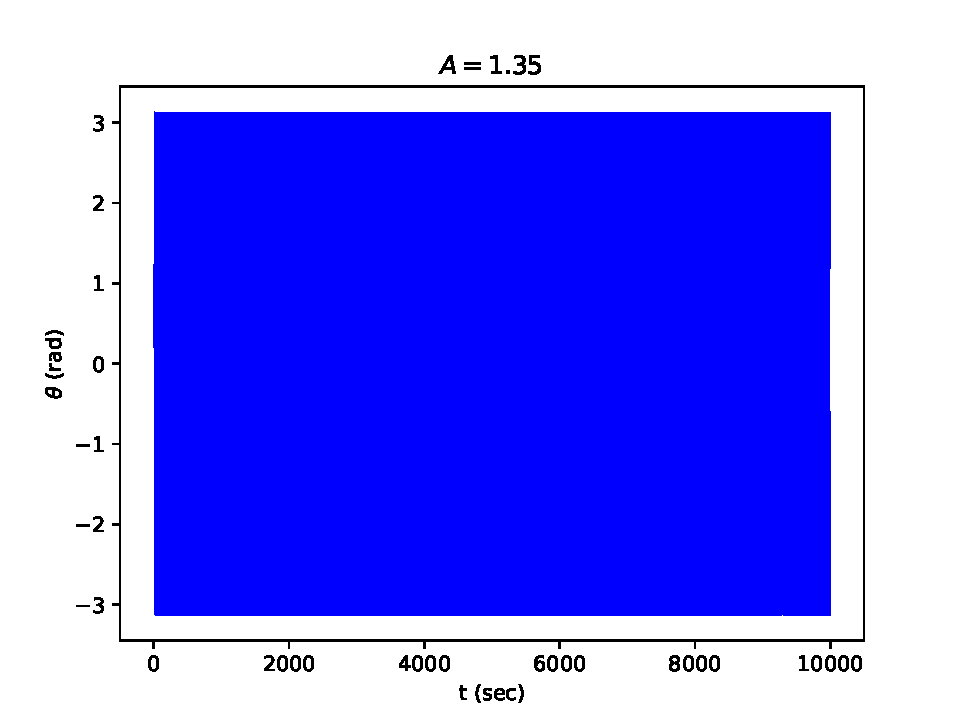
\includegraphics[width=.3\textwidth]{../figs/q4_A_135.pdf}
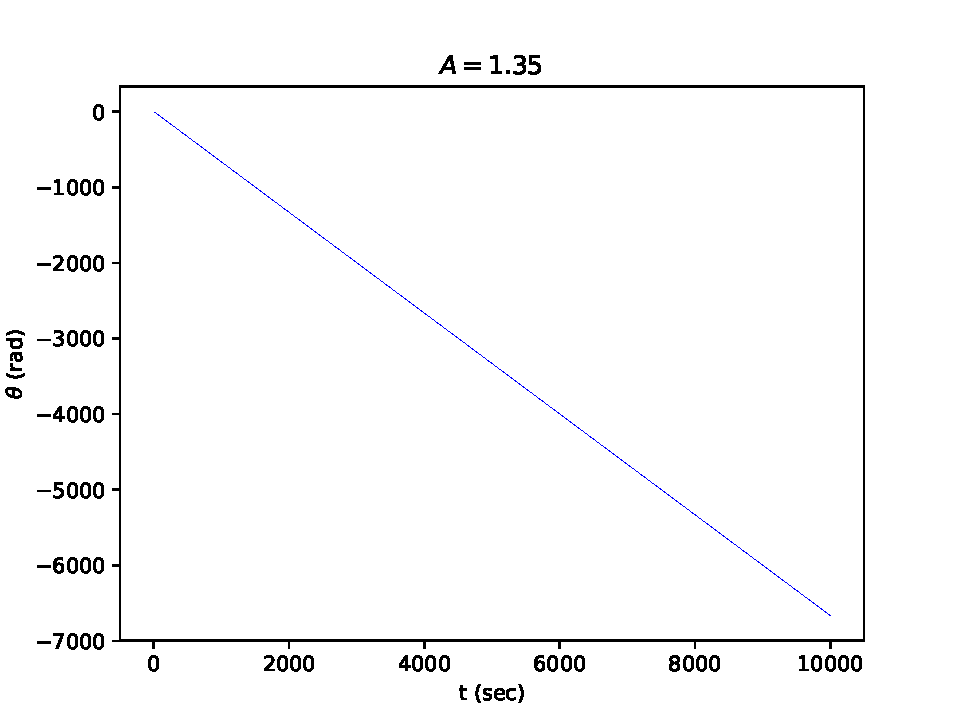
\includegraphics[width=.3\textwidth]{../figs/q4_A_135_no_wrap.pdf}
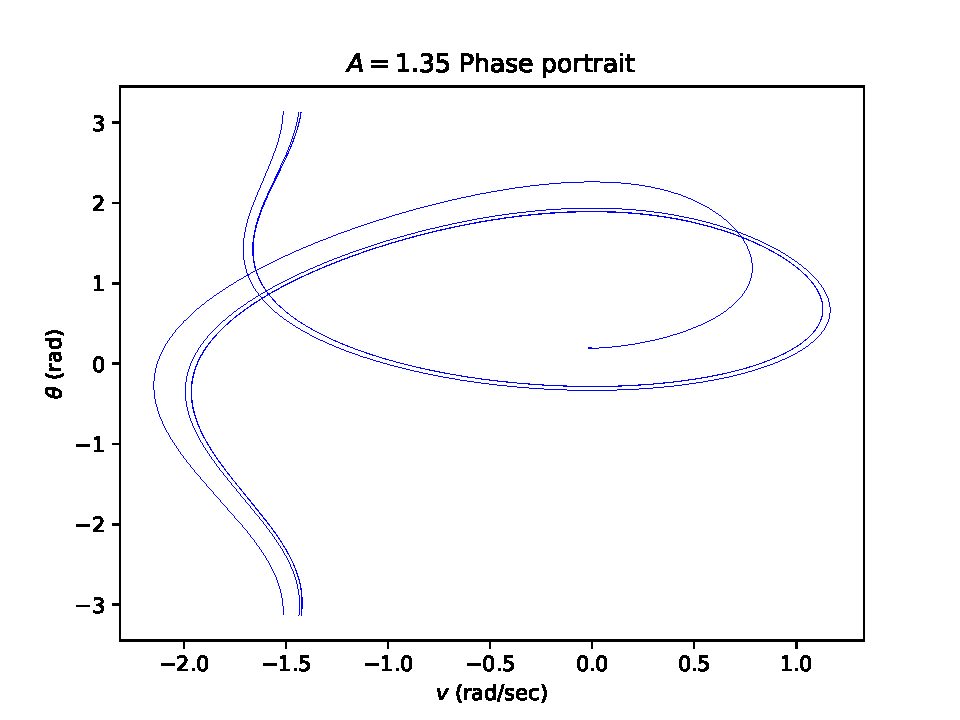
\includegraphics[width=.3\textwidth]{../figs/q4_A_135_phase.pdf}
\end{center}
\begin{center}
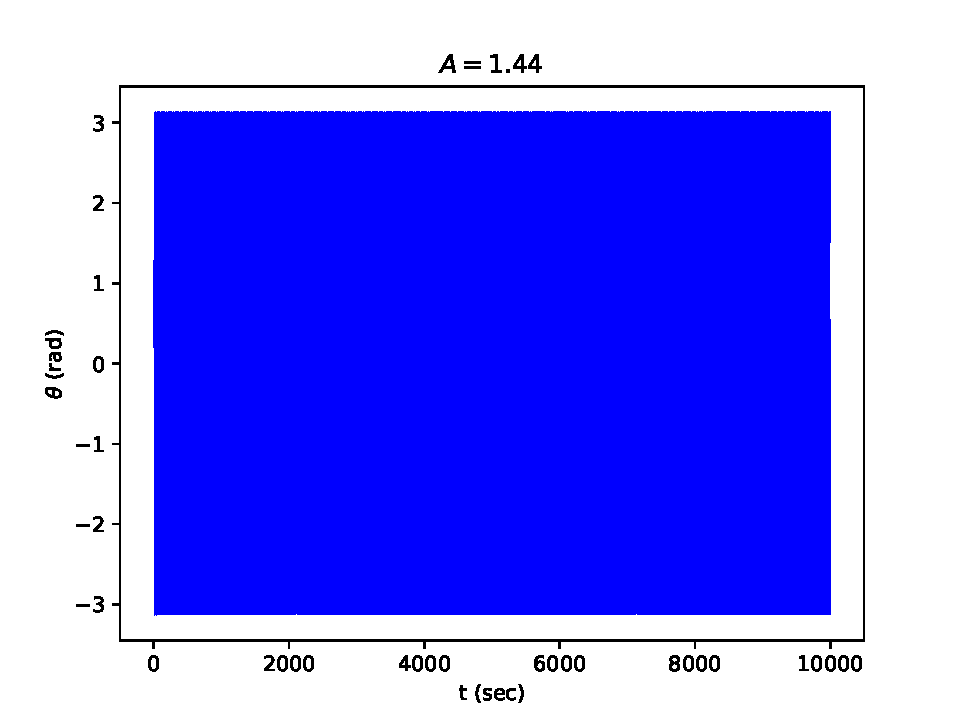
\includegraphics[width=.3\textwidth]{../figs/q4_A_144.pdf}
\includegraphics[width=.3\textwidth]{../figs/q4_A_144_no_wrap.pdf}
\includegraphics[width=.3\textwidth]{../figs/q4_A_144_phase.pdf}
\end{center}
\begin{center}
\includegraphics[width=.3\textwidth]{../figs/q4_A_1465.pdf}
\includegraphics[width=.3\textwidth]{../figs/q4_A_1465_no_wrap.pdf}
\includegraphics[width=.3\textwidth]{../figs/q4_A_1465_phase.pdf}
\end{center}
\noindent \Large{Question 5}
\\ \\
\noindent \normalsize{Please see \texttt{q5.py} in the \texttt{code} folder for relevant code for Q5.}
\\ \\
All chosen $A$'s, except for $A=1.2$, have well-defined values at $n \rightarrow \infty$. As noted earlier, $A=0.5$ and $A=1.33$ have well defined attractors (as seen by their well-defined limit), while $A=1.44$, and $A=1.465$ technically do, but their periodcity for it is much longer than those of $A=0.5$ and $A=1.33$.
\begin{center}
\includegraphics[width=.4\textwidth]{../figs/q5_A_05_Poincare.pdf}
\includegraphics[width=.4\textwidth]{../figs/q5_A_12_Poincare.pdf}
\end{center}
\begin{center}
\includegraphics[width=.4\textwidth]{../figs/q5_A_135_Poincare.pdf}
\includegraphics[width=.4\textwidth]{../figs/q5_A_144_Poincare.pdf}
\end{center}
\begin{center}
\includegraphics[width=.4\textwidth]{../figs/q5_A_1465_Poincare.pdf}
\end{center}
\noindent \Large{Question 6}
\\ \\
\noindent \normalsize{Please see \texttt{q6.py} in the \texttt{code} folder for relevant code for Q6.}
\\ \\
This is a much cleare picture of what is happening. Here we can see that at aroun $A=1.0$, we see period bifurcation leading to chaos. It then should performed period-halving bifurcation to leading to order before $A=1.36$ where it then stays in order up until chaose starts again at around the $A=1.42$ mark. It stay relatively ordered, however, until it reaches around $A=1.48$ where it starts becoming chaotic again.
\begin{center}
\includegraphics[width=.4\textwidth]{../figs/q6_05_12.pdf}
\includegraphics[width=.4\textwidth]{../figs/q6_135_150.pdf}
\end{center}
\end{document}
